% Tipo di documento
\documentclass[10pt, a4paper, twoside]{article}
    \usepackage[english]{babel}
    \usepackage[utf8]{inputenc}
    \usepackage[T1]{fontenc}
%%%%% Pacchetti
\usepackage{imports/packages}		% Pacchetti aggiuntivi di vario tipo (senza tikz)
\usepackage{imports/layout}			% Contiene i pacchetti e le impostazioni per il layout
\usepackage{imports/tikz}				% Ambiente tikzpicture
\usepackage{imports/styles}		% Impostazioni TOC, bibliografia e indice analitico + environments vari per il contenuto del documento
\usepackage{imports/references}		% Collegamenti ipertestuali e indice analitico
\usepackage{imports/custom}			% Comandi vari
%%%%%%%%%%%%%%%%%%%%%%%%%%%%
%%%%%%%%%%%%%%%%%%%%%%%%%%%%

\begin{document}
\title{Titolo}
\author{Paolo Villani\\paolo.villani00@outlook.com}
\date{\today}
\maketitle
\begin{abstractBox}[colbacktitle=black]{Acknowledgements}{
Thanks everyone I didn't make it yet I know you believe in me I will asolutely try my best. My god this will be hard, but I'm on a good way.
}
\end{abstractBox}

\vspace{.5cm}
\pagestyle{fancy}
\pagestyle{fancyfront}

\pagestyle{fancymain}
\newpage
\tableofcontents
%%%%%%%%%%%%%%%%%%%%%%%%%%%%
%%%%%%%%%%%%%%%%%%%%%%%%%%%%
\newpage
\section{Introduction} \label{sec:intro}

When dealing with real-world phenomena, adopting a mathematical representation is often necessary in order to simplify complexity, obtain insight about underlying features, and produce sufficiently accurate predictions on the behaviour of the considered portion of reality. 

In the present day, computer simulations and scientific computing have become essential parts of mathematical modeling, rendering it possible to adopt numerical techniques to solve analytically untractable problems.
Moreover, as numerous and vast families of mathematical models are available to adequately represent different classes of processes, the modeler is presented with choices about model complexity and desired characteristics, as well as with tasks such as parameter identification, model order reduction and uncertainty quantification. 
This work involves all three of these tasks in different manners and measures. 

The problem of the calibration of parameters for a computationally expensive numerical model is considered: a Bayesian perspective is adopted in formulating the inverse problem, and then the cost of model evaluation is reduced by considering a regression-based surrogate model, instead of classical model order reduction techniques such as Proper Orthogonal Decomposition or Reduced-Basis methods.
The considered regression techniques are Gaussian process regression (GPR), which is commonly employed in Bayesian Inverse Problems as it provides not only a pointwise estimate but also a quantification of its confidence, and Lipschitz regression (LR), which is a less utilized technique that also provides a stochastic prediction but relies on different assumptions than GPR. 

To understand the motivation behind this work, it is necessary to provide a brief introduction to the setting in which it is situated.

\subsection{Context and motivation}\label{sec:context}

Inverse Problems (IP) involve the identification of some unidentified quantities in a model through a number of measurements.

We consider a finite dimensional parameter space $\Theta$, a finite dimensional measurement space $ \mc Y$ and the parameter-to-observation map 
\[
 y : \Theta \longrightarrow \mc Y, 
\]
which to each parameter value associates the corresponding measured quantity.

The map implicitly depends on an associated model: we assume the underlying model to be a Partial Differential Equation (PDE) model, which can be evaluated through a Finite Element (FE) discretization.
For a parametrized solution $u(\cdot;p)$ with $p\in \Theta$, some measurement operator $H$ projects the infinite dimensional solution $u$ into the finite dimensional measurement, 
\[
    y (p) = H(u(\cdot;p)) \in \mc Y.
\]
As the PDE solution $u$ is only available through an inexact numerical evaluation $u_\tau$ up to some tolerance $\tau$, the forward model can only be evaluated approximately, i.e.
\[
    y_\tau (p) = H(u_\tau(\cdot;p)) \approx y(p).
\]

FE simulations are often computationally expensive: in order to reduce computational costs, a surrogate model approximating $y$ is introduced.
For a training set $D = \{(p_i,y_i,\tau_i)\}_{i=1}^n$, with $y_i = H(u_{\tau_i}(\cdot;p_i))$, both GPR and LR can provide a mean prediction and some stochastic error bound. 

GPR assumes a Gaussian process prior $\mc{G} \mc P (\mu, k)$ for the unknown ground truth $y$, with $\mu : \mc P \rightarrow \mc Y$ being some mean function and $k: \mc P \times \mc P \rightarrow \mc Y^* $ being a covariance kernel.
Moreover, it assumes that the error on the numerical evaluations $y_\tau$ is a realization of some normally distributed noise, i.e. 
\begin{equation}\label{eq:GPR-noise}
    y_\tau(p) \ \text{ is a realization of } \ y(p) + \nu_d,  \ \text{ with } \ \nu_d \sim \mc N (0, \Sigma_d^2(\tau)),    
\end{equation}
for some covariance matrix $\Sigma_d^2(\tau)$ which depends on the tolerance $\tau$, with a greater tolerance corresponding to larger variance components.
Thanks to this assumptions, it obtains a predictive Gaussian distribution for unseen values of $y$, and computable analytical formulas for the mean and the variance are given.

LR does not need any prior distributional assumptions on $y$, but instead assumes that $y$ is a Lipschitz function.
The Lipschitz constant can be assumed or estimated from data.
Further, the numerical evaluation error is assumed to be the effect of uniformly distributed noise,  
\begin{equation}\label{eq:LR-noise}
    y_\tau(p) \ \text{ is a realization of } \ y(p) + \nu_d,  \ \text{ with } \ \nu_d \sim U(I_\tau )    
\end{equation}
where $I_\tau$ is an open, connected and centered subset of $\mc Y$ which depends on $\tau$.
With these assumptions, LR provides a predictive uniform distribution for unseen values of $y$, guaranteeing a mean prediction and hard bounds.\medskip

The motivation for considering LR lies precisely in the different assumptions on the evaluation noise, Assumptions~\ref{eq:GPR-noise} and~\ref{eq:LR-noise}, required by the two techniques.
For an underlying FE model, the evaluation error depends mostly on the discretization error which results from the choice of a FE basis.
For adaptive FE, the basis is refined until the prescribed tolerance $\tau$ is not met by an error indicator.
The error indicator often guarantees an hard bound on the discretization error: while this is compatible with Assumption~\ref{eq:LR-noise}, it is incompatible with Assumption~\ref{eq:GPR-noise}, which requires an unbounded support for the evaluation error. 

Additionally, in Assumption~\ref{eq:GPR-noise} the covariance matrix $\Sigma_d(\tau)^2$ is often assumed to be diagonal, resulting in independent noise components. 
This ignores any correlation between error components, while the discretization error has some structure due to the underlying FE system.
Hoping to improve the quality of GPR's prediction we introduce and adapt to the given context linear shrinkage estimators, aiming at recovering the underlying error structure. \medskip

For surrogates of both kinds, the IP is reformulated in order to account for the uncertainty introduced by the surrogate model.
A marginal likelihood is derived for both GPR and LR surrogates, and a surrogate-based posterior distribution is obtained.
To select training points, we consider an adaptive training strategy which aims at spending the least computational budget possible in order to obtain a surrogate model with a given accuracy under a certain metric.
We adopt a sequential Design of Experiments (DoE) approach, where the training set is iteratively updated by adding new training points $(p,\tau,y)$, with $p$ being the position of the training point, $\tau$ being the evaluation tolerance and $y$ being the corresponding numerical evaluation.
The considered strategy is goal-oriented, meaning that the training set is adapted to the IP task at hand; it is adaptive, in the sense that not only the position $p$ of the training points $(p,\tau,y)$ is optimized but also the evaluation tolerance $\tau$; and it inverleaves the selection of the training points and updating of the model with the sampling of the posterior distribution over $\Theta$, thus providing a solution to the IP task at hand at the same time as the surrogate model is trained. \medskip

A priori it is not clear if the seemingly more suitable assumptions of LR lead to similar or even better performance than the well-established GPR in the context of IP; similarly, the impact of retrieving the covariance structure of the discretization error on the performance of GPR can hardly be predicted.
Consequently, the final part of this work is dedicated to a number of numerical experiments, where the adaptively trained surrogates are tested on a number of different problems and compared to position adaptive and non adaptive training strategies.
Three different forward models with associated PDEs are considered: for the first two an analytical solution is available, rendering it possible to run a great number of training simulations and to evaluate the ground truth error; for the third one a more realistic model based on an elastomechanics problem is considered, requiring a FE discretization.\medskip

The contributions of this work can be summarized as follows: first, the LR technique will be formalized and generalized, explicitly considering its assumptions and providing a clear framework for its application in the context of IP; second, the formulation of a surrogate-based posterior distribution will be provided in a general form, explicitly stating the marginal likelihood to the LR case; third, an adaptive training strategy for stochastic surrogate models within a DoE framework will be proposed and new error metrics will be stated, extending preceding work to LR-based surrogates and including the estimate of the covariance structure of the discretization error for GPR-based surrogates; finally, a number of numerical experiments will be presented, comparing the performance of GPR and LR surrogates and the impact of the covariance structure of the discretization error on the performance of GPR-based surrogates.\medskip

The remainder of this work is organized as follows: in Section~\ref{sec:context} the context of the work is presented, with first an introduction to Bayesian Inverse Problems and their solution techniques, and then a discussion of Partial Differential Equations and Finite Element discretization.
In Section~\ref{sec:surrogates} the two surrogate techniques are introduced, presenting the established GPR and developing in generality LR, with a discussion of the assumptions made on the data and the model.
In Section~\ref{sec:likelihoods}, the IP is reformulated to account for the surrogate model, and the marginal likelihood is derived for both GPR and LR surrogates.
Section~\ref{sec:AL} presents the adaptive training strategy, first in a general form and then in the specific case of GPR and LR surrogates.
In Section~\ref{sec:exp} three different numerical experiments are presented, comparing the performance of GPR and LR surrogates; a final section regarding the impact of the covariance structure of the discretization error on the performance of GPR-based surrogates is also included.
Finally, in Section~\ref{sec:conclusions} conclusions are drawn and future work is discussed.

\subsection{Related work}\label{sec:literature}

\newpage
\section{Preliminaries} \label{sec:preliminaries}

In the remainder of this section Section~\ref{sec:BIP} first introduces the basic concepts of Inverse Problems and then presents the Bayesian approach to IP, providing a general framework for the formulation of Bayesian Inverse Problems (BIPs) and the derivation of the posterior distribution of the unknown given the observations; Section~\ref{sec:IP-sol} presents some key techniques for the solution of IPs and their numerical treatment, with a focus on the Bayesian approach; Section~\ref{sec:PDE} introduces the basic concepts of Partial Differential Equation (PDE) models, with a focus on the Laplace equation, the diffusion equation and elastomechanic equations as they are the PDEs used in the numerical experiments of Section~\ref{sec:exp}; finally, Section~\ref{sec:AdaFE} presents the Finite Element (FE) method and its adaptive version, which is the solution method for PDEs considered throughout this work.

\subsection{Bayesian Inverse Problems}\label{sec:BIP}

The main reference for this section and the following is Tim Sullivan's Introduction to Uncertainty Quantification~\cite{Sullivan2015}, and other sources will be quoted when utilized. \medskip

Inverse Problems (IP) deal with the identification of some unknown parameter or function in a model through observations of the portion of reality that the model is intended to represent.\newline
Given a measurement $y^m$ in the measurement space $\mc Y$, also known as observation space, the goal of an IP is to identify the pre-image $p*$ in the parameter space $\Theta$ under a map \[y : \Theta \longrightarrow \mc Y \] known as the forward model or parameter-to-observation map.
If a unique $p*$ in $\Theta$ such that
\begin{equation}\label{eq:IP0}
    y(p*) = y^m
\end{equation}
exists, the IP admits a unique solution: but this case is an exception rather than a rule, especially when the observation $y^m$ is corrupted by noise.

A number of techniques have been developed to address from an analytical perspective the numerous issues which arise in an IP.
First, the problem can be reformulated as a least squares problem: for some norm $\| \cdot \| _\mc Y$ on $\mc Y$, Problem~\ref{eq:IP0} is generalized to a minimization problem
\begin{equation}\label{eq:IP1}
    \min_{p\in \Theta} \| y(p) - y^m \|_\mc Y.
\end{equation}
Under regularity conditions such as $\Theta$ and $\mc Y$ being Banach spaces and $y$ being a continuous map, this formulation cannot yet guarantee neither existence, nor unicity, nor stability of a solution $p*$ for every $y^m \in \mc Y$. Nonetheless, Problem~\ref{eq:IP1} is more general as it allows for solutions even if $y^{-1}(\{y^m\} )= \emptyset$, and on the practical side suggests the adoption of optimization techniques to solve IPs.

A second and often compatible approach is that of regularization techniques. 
This involves introducing additional information or constraints to stabilize the solution and make the problem well-posed. Regularization can be performed by the substitution of $y$ with some more treatable operator, or in the case of Variational Regularization by the formulation of a different minimization problem. 
Often, a regularization approach can be understood both from an operator approximation and a variational point of view: this applies to Tychonoff regularization, which can be seen as the addition of a stabilizing term to Problem~\ref{eq:IP1}
\begin{equation}\label{eq:Tycho}
    \min_{p\in \Theta} \big\| y(p) - y^m \big\|_\mc Y^2 + \lambda\big\| p - p^0 \big\|_\Theta^2,
\end{equation}
for some norm $\|\cdot\|_\Theta$ on $\Theta$, $p^0$ in $\Theta$ and $\lambda $ in $ \R^+$. \medskip

As we will see in the next section, both these techniques can be understood by adopting a statistical perspective to IPs, which considers observations corrupted by noise with random behavior and known distribution.
A parameter-to-observation relation is assumed, rendering the available observation $y^m$ a realization of a random variable $Y^m$ over the measurement space $\mc Y$.
We consider an additive noise model
\begin{equation}\label{eq:par-to-obs}
    Y^m = y(p) + N,
\end{equation}
for noise $N$ with distribution $\bb P _N$. \newline
Equation~\eqref{eq:par-to-obs} deals that for any $p$ in $\Theta$, the distribution of $Y^m$ given $p$, noted $\bb P_{Y^m \mid p}$, is given by 
\[
    \bb P_{Y^m \mid p} (A) = \bb P_N (A-y(p))
\]
for any Borel set $A$ in $\mc B (\mc Y)$. 
Note that as $p$ is not a random variable, the distribution $\bb P_{Y^m \mid p}$ is not a conditional distribution and in this context the notation is meant to highlight the dependence of the distribution on the parameter $p$. \newline
For $\mc Y$ of finite dimension, the above equation can be expressed in terms of the probability density functions of $N$ and $Y^m$ with respect to the Lebesgue measure $m_\mc Y$.
As a function of the parameter $p$, the density of $Y^m$ given $p$ is called likelihood and given by
\begin{equation}\label{eq:likelihood}
    L(p) = \pi_{Y^m \mid p} (y^m) = \pi_N(y^m - y(p)).
\end{equation}
The likelihood of a problem is a crucial element in statistical IPs. \medskip

A natural development of the statistical approach to Inverse Problems are Bayesian Inverse Problems (BIPs). 
In the Bayesian setting, the unknown solution $p*$ of the IP is treated as a random variable $P$ and the solution of the IP then becomes the conditional distribution $\bb P_{P \mid Y^m=y^m} $ of $P$ given $Y^m=y^m$.

In full generality, the following result guarantees the possibility of formulating BIPs for arbitrary dimensionality:
\begin{thm} [Regular conditional probability]
    Let $ (\Omega, \mc F , \bb P) $ be a probability space, $\Theta$ be a separable Banach space equipped with the Borel $\sigma$-algebra $\mc B (\Theta)$, $(\mc Y, \tilde{\mc F})$ be a measurable space.
    Further, let $Y^m:\Omega \rightarrow \mc Y$ and $P : \Omega \rightarrow \Theta$ be random variables with $P \in L^1(\Omega, \bb P; \Theta) $. \newline
    Then there exists a $\bb P_{Y^m}$-a.s. unique map $\bb P_{P \mid Y^m} : \mc B (\Theta) \times \mc Y \rightarrow [0,1] $ such that :
    \begin{itemize}
        \item $\bb P_{P \mid Y^m}(\cdot, y)$ is a probability density on $\Theta$ for all $y$ in $\mc Y$;
        \item $\bb P_{P \mid Y^m}(A, \cdot)$ is measurable for all $A$ in $\mc B (\Theta)$;
        \item for all $B$ in $\sigma(Y^m)$, $A$ in $\mc B (\Theta)$, it holds that
                \[ 
                \int_B \bb P_{P \mid Y^m}(A, Y^m(\omega)) \ d\bb P(\omega)= \int_B \ind_A(P(\omega)) \ d\bb P(\omega).
                \] 
    \end{itemize}
    Such map is known as the regular conditional probability of $P$ given $Y^m$ and any map satisfying the first two properties is called a Markov kernel.
\end{thm}

This results guarantees the well-definiteness of conditional probabilities in a general setting, thus allowing for the formulation of BIPs in arbitrary dimensionality, but does not provide a direct way to formulate the posterior distribution given a parameter-to-observation relation. 
This is provided by Bayes' rule, which in generality is given by the following result from~\cite[Theorem 14]{DashtiStuart2017}:

\begin{thm}[Bayes' rule]
    Let $ (\Omega, \mc F , \bb P) $ be a probability space and $\Theta, \mc Y$ be separable Banach spaces equipped with the respective Borel $\sigma$-algebras. 
    Moreover, let $P : \Omega \rightarrow \Theta$ and $N:\Omega \rightarrow \mc Y$ be independent random variables, and $ Y^m = y(P) + N$ with $y: \Theta \rightarrow \mc Y$ a measurable map. \newline
    Assume $\bb P_{Y^m\mid P}(\cdot, p) \ll P_N$ for every $p \in \Theta$, that $\frac{d \bb P_{Y^m\mid P}(\cdot, p)}{d\bb P_N}(y) $ is $\bb P_{(P,N)}$-measurable, and that 
    \[
        \int_\Theta \frac{d \bb P_{Y^m\mid P}(\cdot, p)}{d\bb P_N}(y) \ d\bb P_P(p) > 0 \ \text{ for }  \ y, \ \bb P_N \text{-a.s.}
    \]
    holds.
    Then, the regular conditional probability $\bb P_{P\mid Y^m}(\cdot,y)$ for $P$ given $Y^m$ exists and is such that $\bb P_{P\mid Y^m}(\cdot, y) \ll \bb P _P$ $\bb P_{Y^m}$-a.s., with Radon-Nikodym derivative
    \begin{equation}\label{eq:infdimBayes}
        \frac{d\bb P_{P\mid Y^m}(\cdot, y)}{d\bb P_P}(p) = \frac{1}{Z(y)}\frac{d\bb P_{Y^m\mid P}(\cdot, p)}{d\bb P_{N}}(y).
    \end{equation}
\end{thm}

In the above theorem, $\bb P_P$ is the prior distribution of $P$ and $\bb P_{P \mid Y^m}(\cdot, y^m)$ is then the Bayesian posterior distribution of $P$ given $Y^m=y^m$.
As in~\cite[Theorem 6.31]{Stuart2010}, under certain hypothesis over the measurement space $\mc Y$, the distribution of the noise $\bb P_N$ and the forward model $y$, one has that the conditions over $\frac{d \bb P_{Y^m\mid P}(\cdot, p)}{d\bb P_N}(y)$ hold, rendering the application of the Theorem possible. \medskip

As for the scope of this work it is not necessary to work in full generality, now and for the rest of this work on it will be assumed that the involved spaces $\Theta, \  \mc Y$ are finite dimensional Banach spaces, and that $P$ and $Y$ are random vectors that admit a joint probability density function $\pi_{P,Y}$ with respect to the Lebesgue product measure $m_\Theta \otimes m_\mc Y$. 
This allows for a more intuitive and direct formulation of the Bayesian posterior distribution of $P$ given $Y=y^m$ by exploiting the conditional probability density.

\begin{thm}[Bayes' rule with Lebesgue measure]
    Let $Y = y(P) + N$ hold, with $P$ and $N$ independent and $y: \Theta \rightarrow \mc Y$ a measurable map.
    Then the conditional density of $Y^m$ given $P$ coincides with the likelihood~\eqref{eq:likelihood}, \[
        \pi_{Y^m\mid P = p}(y^m) = \pi_{N}(y^m - y( p) ) = L(p),
    \] and the posterior distribution of $P$ given $Y^m=y^m$ is given by the probability density \begin{equation}\label{eq:Bayes}
        \pi_{P\mid Y^m = y^m}(p) = \frac{\pi_{N}(y^m - y( p) ) \pi_P(p)}{\pi_{Y^m}(y^m)},
    \end{equation}
    where $\pi_{Y^m}(y^m)$ is the marginal density of $Y^m$ given by
    \[
        \pi_{Y^m}(y^m) = \int_\Theta  \pi_{N}(y^m - y( p) ) \pi_P(p) \ dm_\Theta(p).
    \]
\end{thm}

\subsection{Solutions of Inverse Problems}\label{sec:IP-sol}

What it means to solve an IP depends on its formulation and on the objectives that the solution serves.   
The least-squares formulation~\eqref{eq:IP1}, the regularization approach~\eqref{eq:Tycho} and non-Bayesian statistical IPs usually rely on point estimates; the Bayesian formulation instead can also provide a posterior distribution of the unknown given the observations. \medskip

In a statistical framework, the likelihood~\eqref{eq:likelihood} can be utilized to obtain a point estimate of the unknown $p*$ by Maximum Likelihood (ML) estimation
\begin{equation}\label{eq:ML}
    p^* = \arg \max_{p \in \Theta} L(p),
\end{equation}
which maximizes the likelihood of the observations $y^m$ given the parameter $p$.
As the likelihood often decays rapidly it is common to minimize the negative log-likelihood instead, solving the mathematically equivalent but numerically more stable problem \[
    p^* = \arg \min_{p \in \Theta} -\log L(p).
\]
For normal centered noise $N \sim \mc N(0, \Sigma^2)$, the negative log-likelihood is given by
\[
    -\log L(p) = \frac{1}{2} \| y^m - y(p) \|_{\Sigma^{-2}}^2 + \text{const}
\]
where $\| \cdot \|_{\Sigma^{-2}}$ is the norm induced by the inverse of the covariance matrix $\Sigma^2$ of the noise $N$ and $\text{const}$ is a constant term independent of $p$. 
By inserting the above expression in the minimization problem, we see that the ML estimate is equivalent to the minimization of the least-squares problem~\eqref{eq:IP1} with the choice of the norm $\| \cdot \|_{\Sigma^{-2}}$ on $\mc Y$.
By this, the statistical approach naturally provides both a justification and an interpretation for least-squares in IPs; the same happens to regularization techniques, but to see that we need to consider the Bayesian approach. \newline
Within the Bayesian framework, a point estimate can be obtained by Maximum A Posteriori (MAP) estimation which maximizes the posterior density~\eqref{eq:Bayes} of the unknown $P$ given the observations $Y^m=y^m$
\[
    p^* = \arg \max_{p \in \Theta} \pi_{P\mid Y^m = y^m}(p) = \arg \max_{p \in \Theta} L(p) \pi_P(p),
\]
where in the second equality we omitted the denominator $\pi_{Y^m}(y^m)$ as it is independent of $p$.
For normal centered noise $N \sim \mc N(0, \Sigma^2)$ and normal prior $P \sim \mc N(p_0, \Sigma_p^2)$, if we take the negative logarithm of $\pi_{P\mid Y^m = y^m}(p)$ and omit the constants, we can rewrite the MAP problem as
\[
    p^* = \arg \min_{p \in \Theta} \|y^m - y(p) \|_{\Sigma^{-2}}^2 + \|p - p_0 \|_{\Sigma_p^{-2}}^2.
\] 
This, for $\|\cdot \|_\mc Y = \|\cdot \|_{\Sigma^{-2}}$ and $\|\cdot \|_\Theta = \|\cdot \|_{ \lambda \Sigma_p^{-2}}$ is exactly the Least-Squares problem with Tychonoff regularization~\eqref{eq:Tycho}, allowing us to interpret the regularization term as an expression of prior beliefs over the parameter $p$ and the parameter $\lambda$ as a measure of confidence in the prior.
\medskip


While the point estimates can be significantly cheaper to compute, they do not provide a full characterization of the uncertainty in the solution by themselves.
To obtain a representation of the posterior distribution~\eqref{eq:Bayes} of the parameter $P$ given the observations $Y^m=y^m$, we consider Markov Chain Monte Carlo (MCMC) sampling.
MCMC techniques usually require a greater number of evaluations of the likelihood function and consequently of the forward model, but then provide a set of correlated samples from $\pi_{P\mid Y^m = y^m}$. 
Such a set of samples is particularly useful as it allows for Monte Carlo integration
\begin{equation}\label{eq:MC-integration}
    \bb E _{X \sim \bb P_X} [f(X)] = \int_\mc X f(x) \pi_X(x) \ dx \approx \frac{1}{N} \sum_{i=1}^{N} f(x_i).
\end{equation}
Under certain hypothesis on the generation of the samples $\{x_i\}_{i=1}^N$ from $\bb P_X$, a corresponding version of the Law of Large Numbers can guarantee convergence of the right-hand side to the left-hand side for $N \rightarrow \infty$ for any measurable function $f$ integrable with respect to $\bb P_X$.
For $X = P \mid Y^m = y^m$, Monte Carlo integration allows for the computation of several quantities of interest, such as for example the posterior mean and variance.

The first MCMC technique to be introduced was the Metropolis-Hastings (MH) algorithm, first introduced by~\cite{MetropolisRosenbluthRosenbluthTellerTeller1953} and later generalized by~\cite{Hastings1970}.
As MH includes key concepts that are also present in other MCMC techniques while being fairly simple, we will briefly introduce it here.
MH consists of the following algorithm:

\par\noindent\rule[1mm]{\textwidth}{0.4pt}
\phantomsection \makeatletter\def\@currentlabel{Algorithm }\makeatother\label{algo:MH}
\large{\textbf{Algorithm 1 - Metropolis-Hastings.} } \normalsize
\par\noindent\rule[2mm]{\textwidth}{0.2pt}
\textbf{Require:} $\bb P$ target distribution with density $\pi(p)$, a Markov kernel $\mc K$ with density $q(p \mid p ' )$, initial state $p_0$, $N$ samples to draw.
\par\noindent\rule[2mm]{\textwidth}{0.2pt}
For $i =1, \dots, N$ do: 
\begin{enumerate}
    \item Draw proposal $p_n$ from $\mc K (\cdot, p_{n-1})$
    \item Set acceptance threshold: \[ \alpha = \frac{\pi(p_n) q(p_{n-1} \mid p_n )}{\pi(p_{n-1}) q(p_n \mid p_{n-1} )} \]
    \item Draw $u$ from $\mathcal{U}([0,1])$
    \item If $u > \alpha$ then reject: $p_n \leftarrow p_{n-1}$
\end{enumerate}
\textbf{Return} $p_1, \dots, p_N$.
\par\noindent\rule[3.5mm]{\textwidth}{0.4pt}

We observe that, as the target distribution's density is utilized to compute the acceptance threshold $\alpha$ only through a ratio, it needs to be known up to a normalizing constant: this is crucial for the application in BIPs, where the normalizing constant is given by the marginal density $\pi_{Y^m}(y^m)$ which is usually unknown and whose estimation is usually challenging.
This property is fortunately shared by all MCMC techniques \newline
Similarly to Importance Sampling, MH relies on a proposal distribution $\mc K(\cdot, p)$ to generate samples; the rejection step then guarantees that the target distribution is invariant with respect to the sample chain $\{p_i\}$.
The proposal kernel $\mc K$ is crucial both for guaranteeing the convergence of the chain to the target distribution and for the efficiency of the sampling process. 
A sufficient condition for convergence is the absolute continuity of the proposal with respect to the target, i.e. $\mc K(\cdot, p) \ll \bb P $ for every $p$; however, a proposal tailored to the target will result in a better acceptance rate for new samples and both the convergence velocity and the quality of the samples will be higher. 

A number of techniques has been developed to address the issues related to the quality of the sampling process.
First, instead of fixing the proposal distribution, one can choose a family of kernels $\mc K_\theta$ and then adjust the parameter $\theta$ during the sampling process: for random walk MH, the optimal acceptance ratio balancing the exploration of the parameter space and the acceptance of new samples is around $0.234$~\cite{GelmanGilksRoberts1997}, and the proposal distribution can be tuned to achieve this value.
Second, a burn-in or warm-up period can be introduced in order to avoid transient behavior by allowing the chain to converge to the target distribution before starting to collect samples; this reduces the dependence of the resulting chain on the initial state and can improve the quality of the resulting chain.
Third, convergence diagnostics can be performed to assess the state of the chain's convergence to the target distribution and the mixing of the samples.
A commonly employed diagnostic is the Gelman-Rubin potential scale reduction $\hat R$ introduced by~\cite{GelmanRubin1992}, which utilizes multiple independent chains by computing the variance within each chain and the variance between all chains.
For $i =1, \dots, M$, let $\{ \theta_{j}^i \}_{j=1}^{N} \subseteq \R $ be independent chains of length $N$ and let the mean of each chain and overall mean be 
\[
    \bar \theta^i = \frac{1}{N} \sum_{j=1}^{N} \theta_{j}^i, \quad \text{and} \quad \bar \theta = \frac{1}{M} \sum_{i=1}^{M} \bar \theta^ii.
\]
Then, the between chain variance is given by
\[
    B = \frac{N}{M-1} \sum_{i=1}^{M} (\bar \theta^i - \bar \theta)^2,
\]
while the within chain variance is given by
\[
    W = \frac{1}{M} \sum_{i=1}^{M} \frac{1}{N-1} \sum_{j=1}^{N} (\theta_{j}^i - \bar \theta^ii)^2.
\]
An unbiased estimator of the variance of the target distribution is then given by
\[
    \hat \sigma^2 = \frac{N-1}{N} W + \frac{1}{N}B,
\]
and the potential scale reduction is defined as 
\begin{equation}\label{eq:hatR}
    \hat R = \sqrt{ \frac{\hat \sigma^2}{W} }.
\end{equation}
$\hat R$ quantifies the difference in variance between the different chains and is expected to converge to $1$ from above as the chains converge to the stationary distribution. 
Two common practices, both recommended by~\cite[Chapter 11.4]{GelmanCarlinSternDunsonVehtariRubin2013}, are to consider $\hat R < 1.1$ as a convergence criterion and to split each chain into two halves before computing the potential scale reduction in order to test for adequate mixing of each chain.
For multivariate distributions while generalizations of the potential scale reduction $\hat R$ exist, such as the one proposed by~\cite{BrooksGelman1998}, in practice it is common to consider the potential scale reduction of each component of the parameter vector separately and then to take the maximum value of the potential scale reduction across all components.

Once convergence to the stationary distribution is achieved, the generated samples will be correlated and the effects of autocorrelation need to be taken into account when performing Monte Carlo integration; in fact, the variance of the Monte Carlo estimator~\eqref{eq:MC-integration} will be increased by the presence of autocorrelation as compared to i.i.d. data.
Let $X = (X(t))_{t\in \bb N}$ be a Markov chain with stationary distribution $\bb P_X$, let $f$ be square integrable with respect to $\bb P_X$ and assume that the chain is initialized in the stationary state, i.e. $X(0) \sim \bb P_X$.
Then, the correlation at lag $k$ is defined as
\[
    \rho_k = \frac{\text{Cov}[f(X(0)), f(X(k))]}{\text{Var}[f(X(0))]},
\]
and the chain's autocorrelation time as
\[
    \tau_f = 1 + 2 \sum_{k=1}^{\infty} \rho_k.
\]
Under the hypothesis that the finite-dimensional version of the Central Limit Theorem proved by~\cite{KipnisVaradhan1986} guarantees that 
\[
    \sqrt{\frac{\tau_f}{N}} \left(  \bb E_\pi [f(X(0))] - \frac{1}{N} \sum_{j=1}^{N} f(X(j)) \right) \xrightarrow{d} \mc N(0, \text{Var}[X(0)]).
\]
In particular this implies that, for a finite realization $\{ \theta_j\}_{j=1}^N$ of the$X$, the variance of the mean estimator $\frac{1}{N} \sum_{j=1}^{N} f(\theta_j)$ is not given by $\frac{1}{N} \text{Var}[f(X_1)]$ as in the i.i.d. case, but by $\frac{\tau_f}{N} \text{Var}[f(X(0))]$.
This motivates the introduction of the effective sample size (ESS) of the estimator of $f$ for the samples $\{\theta_j\}_{j=1}^N$ of the chain $X$
\begin{equation}
    \text{ESS}_{\{\theta_j\}}^f = \frac{N}{\tau_X} = \frac{N}{1 + 2 \sum_{k=1}^{\infty} \rho_k} \leq N
\end{equation}
where equality holds if and only if the samples are uncorrelated.
The ESS can be understood as the number of independent samples that would provide an estimator for $\bb E[f(X_1)]$ with the same variance as the correlated samples $\{\theta_j\}_{j=1}^N$, and can be used to assess the quality of the samples generated by the chain.
The larger the autocorrelation time $\tau_f$ the smaller the ESS, requiring more samples achieve a desired certainty level.
In practice, the ESS can be estimated via a batch estimate of the autocorrelation of the samples $\{f(\theta_j)\}_{j=1}^N$ with a truncation the sum at a certain lag $k$; this is often used in practice to estimate the ESS~\cite{Geyer1992}.
If the autocorrelation time is significant, Monte Carlo integration can be rendered more computationally efficient by thinning the chain and keeping only every $h$-th sample, i.e. to consider the samples $\{\theta_{h \cdot l}\}_{l=1}^{N/k}$ instead of $\{\theta_j\}_{j=1}^N$.\medskip

Among MCMC techniques, we mention Ensemble Sampling, whose implementation we will use in the numerical experiments of Section~\ref{sec:exp}.
Ensemble Sampling is introduced by~\cite{GoodmanWeare} as an MCMC technique which guarantees invariance with respect to affine transformation of the parameter space and later generalized.
Ensemble Sampling utilizes an ensemble 
\[
X =(X^1(t), \dots , X^M(t))
\] 
comprising of multiple correlated chains $X^i(t)$ known as walkers.
At step $j$ the walkers are updated sequentially; each walker $X^i$ is updated by drawing a proposal $x^i_P(j+1)$ from a distribution, in this context known as move, which depends on the current state of the ensemble 
\[
  X^i_P(j+1) \sim \mc K\left( \cdot ; x^1(j+1), \dots, x^{i-1}(j+1), x^i(j), x^{i+1}(j), \dots, x^M(j)\right).
\] as in MH, the proposal is then accepted or rejected according to the MH threshold $\alpha$. \newline
The two moves proposed by~\cite{GoodmanWeare} are known as stretch move and walk move.
The first draws a proposal for $X^i$ from the line connecting $x^i(j)$ and the current position $x^k(h_k)$ of another walker $X^k$, for $k \neq i$ randomly selected with $h_k = j$ if $k > i$ and $h_k = j+1$ if $k < i$; a univariate random variable $\Lambda$ of an assigned distribution $\bb P_\Lambda$ is used to select the distance from $x^i(j)$ to $x^k(h_k)$ resulting in the proposal
\begin{equation}\label{eq:stretch-move}
    X^i_P(j+1) \sim x^i(j) + \Lambda \cdot (x^k(h_k) - x^i(j)).
\end{equation}
The second selects a proposal for the walker $X^i$ by drawing sample from a Gaussian distribution centered at $x^i(j)$ and with covariance matrix given by the empirical covariance of a subset of the rest of the walkers,
\begin{equation}\label{eq:walk-move}
    X^i_P(j+1) \sim \mc N\left( x^i(j), \frac{1}{|S|-1} \sum_{k \in S} (x^k(j) - \bar x^S(j))(x^k(j) - \bar x^S(j))^T \right),
\end{equation}
where $S \subseteq \{1, \dots, M\} \setminus \{i\}$ is a subset of the walkers and \[\bar x^S(j) = \frac{1}{|S|}\sum_{k \in S} x^k(j)\] is the mean of the walkers in $S$ at step $j$.
Moves can be combined, randomly picking one or another for each walker at each step, and can be parametrized and tuned to improve the acceptance rate of the proposals.

As the posterior distribution could potentially exhibit multimodal behavior, besides the two moves above we will also adopt the Differential-Independence Mixture Ensemble (DIME) move introduced by~\cite{Boehl}, which combines Ensemble Sampling with ideas from the Differential Evolution MCMC framework introduced by~\cite{TerBraak} and behaves efficiently on multimodal distributions. 
The DIME move divides the ensemble in two subsets of similar size and updates one using a local proposal, the Differential Evolution proposal from~\cite{TerBraak}, and the other using a global proposal with heavy tails, a parametrized multivariate t-distribution.
Thanks to its adaptivity, the DIME move is able to explore the parameter space and to sample efficiently from multimodal distributions without sacrificing the effectiveness on unimodal distributions.

\subsection{Partial differential equation models} \label{sec:PDE}

For this section and the following, we will use Peter Deuflhard and Martin Weiser's Adaptive Numerical Solution of PDEs~\cite{DeuflhardWeiser2012} as a reference; other sources will be quoted when utilized.

Partial differential equations (PDEs) are a class of equations that relate a function of several variables to its partial derivatives.
For a sufficiently smooth function $u : D \rightarrow \R^o$ defined on an open domain $D \subseteq \R^l$, a differential equation of degree $k$ can be first represented as an equation of the form
\[
    F\big(,u(x), \nabla u(x), \nabla^2 u(x), \dots, \nabla^k u(x)\big) = 0,
\]
for a function $F: D \times \R^o \times \R^{o \times l} \times \dots \times \R^{o \times l^k} \rightarrow \R^e$.
If $l =1$, then all the derivatives are univariate and the equation is ordinary differential equation (ODE), while if $l > 1$ the equation is a proper PDE.

A first distinction that can be introduced is that between time-dependent and non time-dependent PDEs.
In fact, despite the fact that the definition of a PDE does not make a distinction between time and space variables, it is often useful for use cases to distinguish between the two.
For the rest of this chapter and the following, $D$ will indicate a generic domain, $\mc X$ will indicate the space-domain of dimension $l$, while $\mc T$ will indicate the time-domain and $t$ will denote a time variable; for time-dependent PDEs the domain will thus be $\mc T \times \mc X$ and the functions $u(t,x)$, while for non time-dependent PDEs the domain will be $\mc X$ and the functions $u(x)$.
A second distinction is that between linear and non-linear PDEs: a PDE is linear if the function $F$ is affine with respect to the unknown function $u$ and its derivatives.
We will only deal with linear PDEs: non linear PDEs are usually more difficult to treat  than linear PDEs, and in many cases they can be approximated by linear PDEs.

Like in ODEs, the solution of a PDE is in usually non unique unless additional information is provided; this information is usually provided in the form of boundary conditions on $\mc X$, which lead to a boundary value problem, in the form of initial conditions on $\mc T$, which lead to an initial value problem, or combining the two.
Unlike ODEs, where the existence and uniqueness of the solution depends on the regularity of the function $f$ around the initial condition, in PDEs the existence of a solution can be more complicated and issues of compatibility between the boundary conditions and the equation can arise.
Moreover, for a PDE different kinds of boundary conditions can be imposed, and we consider three main types of boundary conditions: Dirichlet, Neumann and Robin boundary conditions.
For a subset $B \subseteq \bar D$ of the domain, Dirichlet boundary conditions impose the value of the solution on $B$, i.e.
\[
    u(x) = g(x), \quad \forall x \in B,
\]
for some function $g: B \rightarrow \R^o$;
Neumann boundary conditions impose the value of the normal derivative of the solution on $B$, i.e.
\[
    \partial_{\hat{n}} u(x)= \hat n \nabla u(x) = g(x), \quad \forall x \in B,
\]
where $\hat n$ is the unit normal vector on the boundary $B$; 
finally, Robin boundary conditions impose a linear combination of the value of the solution and its normal derivative on $B$, i.e.
\[
    \partial_{\hat{n}} u(x) + \alpha(x) u(x) = g(x), \quad \forall x \in B.
\]
We will now proceed to introduce some exemplary linear PDEs, which will then be used in the numerical experiments of Section~\ref{sec:exp}.\medskip

The first one is the Poisson equation, given by 
\begin{equation}\label{eq:Poisson}
    -\Delta u(x) = f(x), 
\end{equation}
over a domain $\mc X \subseteq \R^l$, where $\Delta$ is the Laplace operator, defined as the divergence of the gradient of $u$, 
\[
    \Delta u(x) = \nabla \cdot \nabla u(x) = \sum_{i=1}^{l} \partial^2_{x_i} u(x), 
\] and $f$ is a given scalar function on $\mc X$.
The Poisson equation is a second-order linear PDE and is the simplest representative of elliptic PDEs and is used to model a variety of phenomena, such as heat conduction, electrostatics and fluid flow; its homogeneous version, i.e. with $f=0$, is known as Laplace equation and the solutions of the Laplace equation are known as harmonic functions.

A general solution for the Poisson equation can be derived by the method of Green's functions, which consists in representing the solution as the sum of the convolution of the right-hand side $f$ with a Green's function $G(x,y)$ plus a boundary term~\cite[Chapter 2.2, Theorem 12]{Evans2010}.
Obtaining Green's function is usually a non-trivial task, as it depends on the domain $\mc X$ and the boundary conditions imposed on it.
A crucial element to obtain the Green's function is the fundamental solution of the Laplace equation, which for the 3-dimensional case $l=3$ is given by
\begin{equation}\label{eq:Poisson-fundamental-solution}
    \begin{gathered}
        \Phi : \R^3 \setminus \{0\} \rightarrow \R, \\
        \Phi(x) =  -\frac{1}{4\pi \|x \|_2}.
    \end{gathered}
\end{equation}
The fundamental solution $\Phi$ is harmonic on $\R^l\setminus \{0\}$ and can be derived as a rotationally invariant solution of the Laplace equation.
The key property of the fundamental solution is that the equation 
\[ 
    \Delta \int_{\R^l} \Phi(x-y) f(y) \ dy = f(x) 
\]
holds for every $x \in \R^l$ and $f \in \mc C^2_c(\R^l)$ twice continuously differentiable with compact support~\cite[Theorem 1]{Evans2010}.
This justifies writing \[
    \Delta \Phi(x) = \delta(x),
\]
i.e. the Laplace operator of the fundamental solution is equal to Dirac's delta distribution $\delta$.
Green's function is then defined by 
\[
    G(x,y) = \Phi(y-x) + h_x(y),
\]
where $h_x(y)$ is an harmonic corrector term which guarantees the satisfaction of the boundary conditions imposed on the domain $\mc X$. \medskip

The second type of PDE we will consider is the diffusion or heat equation, given by
\begin{equation}\label{eq:diffusion}
    \partial_t u - k \Delta u = f,
\end{equation}
on some domain $\mc T \times \mc X$, with $k\in \R^+$ a positive constant and $f$ a given function on $\mc T \times \mc X$ and the Laplacian $\Delta$ acting on the spatial variable $x$.
The diffusion equation is a time-dependent second-order linear PDE and is used to model the diffusion of a quantity $u$ in time and space, such as heat or the concentration of a substance.
$f$ is known as the source term and can be used to model the presence of a source or sink of the diffusing quantity $u$, while $k$ is known as the diffusion coefficient and describes the rate at which the quantity diffuses in space; it is usually assumed to be positive as negative values can be understood as an inversion of the time direction.

Similarly to the Poisson equation, the diffusion equation admits a fundamental solution given by
\[
    \begin{gathered}
        \Phi : \R^l \times \R \rightarrow \R, \\
        \Phi(x,t) = 
        \begin{cases}
            \frac{1}{(4\pi k t)^{l/2}} e^{-\frac{\|x\|_2^2}{4kt}} & \text{for } t > 0 \\
            0 & \text{for } t \leq 0.
        \end{cases}
    \end{gathered}
\]
The fundamental solution of the heat equation can be considered the solution of the initial value problem 
\[
    \begin{cases}
        \partial_t u - k \Delta u = 0 & \\
        u(0,x) = \delta(x). &
    \end{cases}
\]
over $\R^+ \times \R^l$ and has the property that solutions of various problems on the heat equation can be solved by convolution of a term with the fundamental solution~\cite[Chapter 2.3, Theorem 1-2]{Evans2010}.


\subsection{Adaptive Finite Element method} \label{sec:AdaFE}
\newpage
\section{Stochastic surrogate models}\label{sec:surrogates}
To reduce the computational costs related to the evaluation of the forward model, a surrogate model is an attractive option.
The scope of the surrogate model is to approximate the forward model $y : \Theta \rightarrow \mc Y $ or the problem's likelihood $L: \Theta \rightarrow \R $ directly with a simpler and faster model.\newline

Whether the surrogate aims at representing the forward model or the likelihood directly is a matter of convenience.
Producing a surrogate representation of the forward model guarantees a cheaper representation of the likelihood, but not vice versa. Moreover, the values the likelihood assumes are constrained to be positive, which can be non-trivial to impose for certain classes of surrogates; however, an argument in favor of adopting a surrogate for the likelihood is that, if the forward model has a great number of output components, the computational costs of a likelihood surrogate can be significantly lower than the ones of a forward model surrogate.

Ultimately, the choice of the target of the surrogate model depends on the adopted surrogating technique, the usage of the surrogate and the objective being pursued.
When a point estimate of the parameter is a sufficient solution for the IP, adopting a Bayesian Optimization framework and surrogating the likelihood directly is the most natural choice.
Instead, when aiming for a posterior representation through sampling, approaches such as Delayed Acceptance MCMC \cite{ChristenFox2005} are indifferent to the choice.
For the approach presented in this work, a forward model representation will be obtained, as we will exploit the error estimators for FE models in the surrogate's training. \newline

We will consider training data $ D =\{ (p_i, \tau_i, y_i) \}_{i=1}^n $, where $ p_i \in \Theta $ are the input parameters, $ \tau_i \in \R_+ $ are the tolerances of the model's evaluation, and $ y_i \in \mc Y $ are the output values of the numerical forward model,\[ y_i = H(f_{\tau_i}(\cdot; p_i)). \]

There exist different classes of surrogate models: an useful distinction is the one between deterministic and stochastic surrogate models.
Deterministic surrogate models are based on deterministic functions, such as polynomial regression, neural networks, or support vector machines.
They provide an approximation of the forward model or the likelihood, but they do not provide by default an estimate of their own uncertainty.
On the other hand, stochastic surrogate models are based on probabilistic assumptions and naturally provide an estimate of the uncertainty associated with their prediction.
This is particularly useful in the context of BIPs, as the uncertainty of the surrogate model can be incorporated in to the problem's likelihood, as illustrated in Sections~\ref{sec:GPlike} and~\ref{sec:LRlike}. \newline

We will adopt stochastic surrogate models, which for any $p \in \Theta$ provide a random prediction with a certain predictive distribution. 
The surrogate model could thus be viewed as a stochastic process, but as this is not necessary for the scopes of this work, we see it as a function that to each parameter $p$ associates a probability distribution $ P( y(p) \mid D)$ in the set $\mc P (\mc Y)$ of probability distributions over $\mc Y$.
For training data $D$, we write \begin{align*}
    y_D : \Theta \rightarrow \mc P( \mc Y) \\
    p \mapsto \bb P( y(p) \mid D).
\end{align*}

In the next two section, we introduce two techinques which provide a stochastic surrogate model: Gaussian process regression (GPR) and Lipschitz regression (LR).

\subsection{Gaussian process regression}\label{sec:GPR}
Gaussian process regression (GPR) is a non-parametric regression technique which relies on probabilistic assumptions and is closely related to support vector machines and kernel methods.

The core idea is that the underlying function $y$ is a realization of a Gaussian process and, assuming the observation are contaminated by Gaussian noise, GPR obtains a closed-form prediction through Gaussian conditioning.\newline

\begin{dfn} [Gaussian Process]
    A Gaussian process (GP) over $\mc Y$ is a collection $Y = \{Y_p\}_{p\in\Theta}$ of $\mc Y$-valued random variables, such that for any finite subset $p_1, \ldots, p_n \in \Theta$, the random variables $Y_{p_1}, \ldots, Y_{p_n}$ have a joint Gaussian distribution.

    A Gaussian process is completely defined by its mean function $m: \Theta \rightarrow \mc Y$ and its covariance function $k: \Theta \times \Theta \rightarrow SPSD_{\text{dim}\mc Y}(\R)$, also known as kernel. 
    We denote $Y \sim GP(m, k)$ for a Gaussian process of mean $m$ and kernel $k$.
\end{dfn}
Note that the covariance operator $k(p, p')$ can be identified with a positive semidefinite matrix as $\mc Y$ is of finite dimension. \newline

Gaussian process regression relies on two assumptions:
\begin{itemize}[font=\itshape, leftmargin=1.5cm, align=right, labelwidth=2.4cm]
    \item[(GPR-model)] the forward model $y$ is a realization of a GP $Y \sim GP(m, k)$;
    \item[(GPR-data)]the observations are contaminated by Gaussian noise independent from $Y$, i.e. 
    \[ 
        y_i = y(p_i) + e_{D,i} \ \text{ for every } \ (p_i,\tau_i,y_i) \ \text{ in } \ D 
    \] 
    holds, where $e_{D,i} \sim \mc N(0, \Sigma_D(\tau_i)^2)$ for some $\Sigma_D(\tau)$, and $e_{D,i}$ is independent from $Y$.
\end{itemize}  
The first assumption implicitly prescribes a certain regularity of the forward model depending on the choice of the kernel $k$, but does not impose any parametric form on the model itself. 
The choice of a kernel is crucial for the effectiveness of GPR: in order to allow for flexibility, in practice a parametric family of kernels $\{ k_\lambda\}$ is chosen to model the covariance, with $\lambda$ known as the kernel's hyperparameters. More remarks about kernel structure and hyperparameters will be made at the end of this section. \newline
The second assumption allows to derive a closed-form expression for the predictive distribution of the GP, and in our context entails that the discretization error on numerical evaluations of the forward model is Gaussian, i.e. \[
    H(f_{\tau}(\cdot; p)) - H(f(\cdot; p)) \sim \mc N(0, \Sigma_D(\tau)^2);
\] for a general GPR task, it is common to assume 
\begin{equation}\label{eq:iid-GPR-noise}
    \Sigma_D(\tau) = \tau I_{\text{dim} \mc Y}
\end{equation} 
and often $\tau$ is unknown and fitted together with the kernel's hyperparameters. \newline
In the context we are working in, Equation~\eqref{eq:iid-GPR-noise} implies i.i.d. components of the FE discretization error, which is not realistic: Section~\ref{sec:GPAL} presents an approach to model the discretization error covariance by exploiting an adaptive FE scheme. \newline

Given a prior GP $Y \sim GP(m, k)$ and the training data $D$, the posterior GP $Y \mid D$ is obtained by conditioning the prior on the observations. 
The analytical expression for the posterior GP is given by the following theorem.
Although this result is foundational for GPR, its complete proof is rarely explicitly stated.~\cite[Appendix A]{RasmussenWilliams2006} provides the necessary results for the full proof, which we will present explicitly in Appendix~\ref{app:GPR}.

\begin{restatable}[GP posterior]{theorem}{GPpost} \label{thm:GP-posterior}
    Under assumptions \textit{(GPR-model)} and \textit{(GPR-data)}, assume that the covariance between the noise terms $e_{D,1},\dots,e_{D,n}$ is given by some positive definite $\Sigma_D(\mc T)^2$ for $\mc T = (\tau_1, \ldots, \tau_n)$. \newline
    Then the posterior GP $Y \mid D$ is a GP over $\mc Y$ with mean function $m_D$ and kernel $k_D$, where
    \begin{gather}
        m_D(p) = m(p) + k(p, P) (k(P,P) + \Sigma_D(\mc T)^2 )^{-1} (y - m(P)) \label{eq:predictive-mean} \\
        k_D(p, p') = k(p, p') - k(p, P) (k(P,P) + \Sigma_D(\mc T)^2 )^{-1} k(P, p')^T \label{eq:predictive-var}
    \end{gather}
    for $P = (p_1, \ldots, p_n)$ and block matrices $K(P,P)_{i,j} = k(p_i, p_j)$, and $k(p, P) = (k(p, p_1), \ldots, k(p, p_n))$.
\end{restatable}

As we are not interested in the full GP posterior but only in the point-wise predictive distribution, the following corollary allows us to define the GPR surrogate we will employ.
\begin{cor}
    Under the assumptions of Theorem~\ref{thm:GP-posterior}, the GPR predictive distribution given the prior $GP(m,k)$ and the data $D$, is given by 
    \begin{gather*}
        y_{D, \text{GP}} : \Theta \rightarrow \mc P( \mc Y) \\
        p \mapsto \mc N( m_D(p), \sigma_D^2(p) ),
    \end{gather*}
    where $ \sigma_D^2(p) = k_D(p,p)$, with $m_D$ and $k_D$ are given by Equations~\eqref{eq:predictive-mean} and~\eqref{eq:predictive-var} respectively.
\end{cor}

The core of GPR is now outlined, but for practical use a few more remarks are necessary.
As mentioned above, the kernel structure and the treatment of hyperparameters play an essential role in GPR.

The choice of what parametric family of kernels $\{ k_\lambda\}$ to adopt determines the regularity of the GP's mean and realizations, see ~\cite{Kanagawa2018} and~\cite[chap. 4]{ChristmannSteinwart2008}; moreover, the parametrization $\lambda \mapsto k_\lambda$ needs to allow for efficient optimization of the hyperparameters $\lambda$. \newline
To ease the hyperparameters optimization problem and improve computational efficiency, the kernel $k_\lambda$ is often chosen to be stationary, i.e. 
\[
k_\lambda(p, p') = g_\lambda(p - p') \ \text{ for every } \ p, p' \in \Theta
\]
for some $g_\lambda:\Theta \rightarrow \R$.
For dim$\mc Y > 1$, it is common to model the correlation between inputs and outputs separately~\cite{AlvarezRosascoLawrence2012}; this results in what is known as a separable kernel \[
    k_\lambda(p, p') = \kappa_{\lambda_i}(p, p') K_{\lambda_o}
\] for $\lambda = (\lambda_i, \lambda_o)$, with $\kappa_{\lambda_i}: \Omega \times \Omega \rightarrow \R$ and $K_{\lambda_o} \in R^{m\times m}$ being a scalar kernel and a symmetric positive definite matrix.
$\kappa_{\lambda_i}$ models the correlation between different inputs and $K_{\lambda_o}$ models the correlation between output components.

The possible choices for families of kernels are vast and it is important to note that sums and products of kernels are again kernels, allowing for the construction of complex kernel structures by the combination of elementary kernels~\cite{Duvenaud}.
Among such elementary kernels, particularly relevant are the Radial Basis Function (RBF) kernel and the Matérn kernel. \newline
The expression of the RBF kernel, also known as squared exponential kernel, is given by
\[
k_{\lambda}(p, p') = \exp\left(-\frac{\|p - p'\|_\Theta^2}{2\lambda^2}\right),
\]
with $\lambda$ being a length-scale parameter. 
Note that more complex RBF kernels can be obtained by altering the norm $\| \cdot \|_\Theta$, and for a parametrized norm this leads to what is known as Automatic Relevance Determination (ARD).
The RBF kernel leads to a $\mc C^\infty$ mean prediction and is usually adopted as a default choice whenever the underlying function can be assumed to be rather smooth. \newline
The Matérn kernel allows for less-regular predictions. Its general expression is given by
\[
k_{(\nu, \lambda)}(p, p') = \frac{2^{1-\nu}}{\Gamma(\nu)} \left( \frac{\sqrt{2\nu} \|p - p'\|}{\lambda} \right)^\nu K_\nu \left( \frac{\sqrt{2\nu} \|p - p'\|}{\lambda} \right),
\]
where $\Gamma$ is the Gamma function $K_\nu$ is a modified Bessel function~\cite[sec. 9.6]{AbramowitzStegun1964};
for $\nu = n + \frac{1}{2}$ with $n\in \bb N$, the expression simplifies to 
\[
     k_{n+\frac{1}{2}, \lambda}(p, p')=\exp \left(-{\frac {{\sqrt {2n+1}}\|p - p'\|}{\lambda }}\right){\frac {n!}{(2n)!}}\sum _{i=0}^{n}{\frac {(n+i)!}{i!(n-i)!}}\left({\frac {2{\sqrt {2n+1}}\|p - p'\|}{\lambda }}\right)^{n-i}.
\]
The regularity of the predictive mean depends on the parameter $\nu$: the mean prediction is $\nu + \frac{1}{2}$-times weakly differentiable.
Most commonly, $\nu$ is set to $\frac{3}{2}, \frac{5}{2}$ or $\frac{7}{2}$, as $\nu = \frac{1}{2}$ leads to a non-differentiable mean prediction, and for $\nu > \frac{7}{2}$ the high regularity favors the adoption of a RBF kernel.
Note that for $\nu \rightarrow \infty$ the Matérn kernel converges to the RBF kernel. \newline

The treatment of hyperparameters constitutes an estimation problem.
For training data $D =\{ (p_i, \tau_i, y_i) \}_{i=1}^n$, the distribution of the data given the hyperparameters $\Lambda = \lambda$ is given by
\[
    (Y_{p_1}, \dots, Y_{p_n}) \mid \Lambda \sim \mc N \left( (m(p_1), \dots, m(p_n)), k_\lambda(P,P) + \Sigma_D(\mc T)^2 \right)
\]
with $k(P,P)$ and $\Sigma_D(\mc T)$ as given in Theorem~\ref{thm:GP-posterior};
this results in the hyperparameters' likelihood given the data,
\[
    L(\lambda) = \pi_{(Y_{p_1}, \dots, Y_{p_n}) \mid \Lambda} \big ( (y_1,\dots,y_n) \mid \Lambda = \lambda \big ).
\]
To solve the problem, one either adopts a point estimate, given usually by ML or MAP, or marginalizes the GPR prediction over the hyperparameter posterior distribution by sampling. 
While marginalizing propagates the uncertainty in the hyperparameters, it is computationally considerably more expensive: due to this reason a point estimate is most commonly employed and one talks about hyperparameter optimization. Gradient-based methods are utilized in the problem's solution. \newline


\subsection{Lipschitz regression}\label{sec:LR}
\newpage
\section{Surrogate-based likelihoods}\label{sec:likelihoods}
\todo[inline]{read again}
Having obtained a stochastic surrogate model $y_D$, we wish to utilize it to evaluate the likelihood of the problem.

A first approach consists of considering the mean prediction of the surrogate model as a response surface and use that in the likelihood~\eqref{eq:likelihood} evaluations. 
For a mean prediction $m_D$, this corresponds to a parameter-to-observation relation 
\begin{equation}\label{eq:plug-in-par-to-obs}
    Y^m = m_D(p) + N
\end{equation}
and results in the likelihood
\begin{equation}\label{eq:plug-in-likelihood}
    L_{\text{plug-in}}(p) = \pi_N(y^m - m_D(p)).
\end{equation}
This is the so-called plug-in likelihood, which is a frequent choice in the literature~\cite{SinsbeckNowak2017}. 

However, this approach does not take into account the uncertainty of the surrogate model, which can lead to overconfident predictions and biased estimates of the parameters.
As we assume to be working with partial knowledge about the forward model $y$ only, our information about the relation between observation and parameters will also be limited. 
Relation~\eqref{eq:par-to-obs} may hold for the true forward map $y$, but as only a set $\{y_i\}_{i=1}^n$ of evaluations up to a certain accuracy is available, it is of little practical use. 
Thanks to the assumptions required by GPR and LR a new relation can be obtained, incorporating the uncertainty about the forward model and resulting in a surrogate-dependent likelihood. 

\subsection{GPR-based likelihood}\label{sec:GPlike}
By the assumptions of Section~\ref{sec:GPR}, when performing GPR one assumes the forward model to be a realization of a Gaussian process $Y$.
Incorporating this into the Relation~\eqref{eq:par-to-obs} leads to a different parameter-to-observation relation
\begin{equation}\label{eq:GPR-par-to-obs}
    Y^m = Y_p + N.
\end{equation}
Under normality and indipendence assumptions this results in a different likelihood, as stated in the following proposition.

\begin{prp}
    Let Relation~\eqref{eq:GPR-par-to-obs} hold with Gaussian noise $N \sim \mc N (0, \Sigma_N^2)$, let $y^m$ be a realization of $Y^m$ and let $y_{D, \text{GP}}$ be a GPR surrogate model describing the posterior distribution of $Y_p$ given training data $D = \{ (p_i, y_i) \}_{i=1}^n$.

    Under the hypothesis that the GP prediction $Y_p$ is indipendent from the measurement noise $N$, Relation~\eqref{eq:GPR-par-to-obs} yields that $Y^m$ is normally distributed,
    \[
    Y^m \sim \mc N(m_D(p), \Sigma_N^2 + k_D(p,p)), 
    \]
    and consequently the marginal GPR likelihood is given by
    \begin{equation}\label{eq:GPR-likelihood}
        L_{D, \text{GP}}(p) = (2\pi)^{-\frac{\text{dim} \mc Y}{2}} \text{det}\big ( \Sigma_N^2 + k_D(p, p) \big )^{-\frac{1}{2}} \exp \Big( -\frac{1}{2}\norm{y^m - m_D(p)}_{(\Sigma_N^2 + k_D(p,p))^{-1}}^2 \Big ).
    \end{equation}
\end{prp}
\begin{proof}
    \todo[inline]{Proof}
\end{proof}
\begin{rmk}
    The marginal GPR likelihood is the marginal distribution for $Y^m$ of the joint distribution of $Y^m$ and $Y(p)$:
    \begin{equation*}
        L_{D}(p) =  \mathbb E_{Y_p \sim \mc N (m_D(p),k_D(p,p))} \Big [ \pi_N (y^m - Y_p) \Big ].
    \end{equation*}
\end{rmk}

\todo[inline]{maybe rephrase last parts}

As the prediction of GPR is stochastic, it is reasonable that likelihood of observing $y^m$ depends not only on the mean $m_D$, but also on the variance $k_D$. 
This is reflected in the likelihood~\eqref{eq:GPR-likelihood}, which by having an higher variance is less prone to produce an overconfident posterior, but comes at the price of a more complicated likelihood function when compared to the plug-in likelihood~\eqref{eq:plug-in-likelihood}.
Since the covariance of the marginal likelihood depends on $p$, more local minima and non-convex behavior can be present; nonetheless, this can be expected to be less of a problem for sampling-based approaches to IPs than for optimization-oriented approaches.

Picture () compares the plug-in and the marginalized likelihoods for a simple one-dimensional case.
\todo[inline]{picture representing plugin/marginal likelihood}


\subsection{LR-based likelihood}\label{sec:LRlike}

Under the assumptions described in Section~\ref{sec:LR}, we can treat Relation~\eqref{eq:par-to-obs} similarly as done for GPR. 

Remind that, given training data $D =\{ (p_i, \tau_i, y_i) \}_{i=1}^n$, LR provides a predictive uniform distribution over some convex set $\mc PI_p \subseteq \mc Y $.
Marginalizing the likelihood over this predictive distribution leads to a marginal likelihood $L_{D, \text{LR}}(p)$ as given by the following proposition.

\begin{prp}\label{prp:LR-likelihood}
    Let $y_{D, \text{LR}}$ be a LR surrogate model as given in Definition~\ref{dfn:LR}, then if the prediction $Y_p \sim \mc U (\mc IP_p)$ is indipendent from the noise term $N$, the LR parameter-to-observation relation 
    \begin{equation*}
        Y^m = Y_p + N 
    \end{equation*}
    yields the marginal LR likelihood
    \begin{equation}\label{eq:LR-likelihood}
        L_{D, \text{LR}}(p) = \frac{1}{m_\mc Y (\mc PI_p)} \mathbb P \Big ( N \in \mc PI_p - y^m \Big ).
    \end{equation}
\end{prp}
\begin{proof}
    \todo[inline]{Proof}
    \begin{align*}
        \pi\big (y^m \mid L, D, p \big ) &= \int_{\mc P I_p } \frac{\varphi(y^m - y)}{m_\mc Y (\mc PI_p)} \ dy = \\
        & = \frac{1}{m_\mc Y (\mc PI_p)} \int_{\mc P I_p  - y^m} \varphi(e )  \ de  = \frac{1}{m_\mc Y (\mc PI_p)} \mathbb P \Big ( N \in   \mc PI_p - y^m \Big  ). \notag
    \end{align*}
\end{proof}

The efficience in computing the likelihood~\eqref{eq:LR-likelihood} depends on the distribution of the measurement noise $N$ and the shape of $\mc P I_p  $.
For Gaussian measurement noise $N$ with indipendent components and $\mc PI_p$ being a rectangle, the likelihood can be computed as the product of differences of Gaussian cumulative distribution functions, as stated in the next proposition.

\begin{prp}
    In the hypothesis of Proposition~\ref{prp:LR-likelihood}, let  $N \sim \mc N (0, \Sigma^2_N)$ be Gaussian with $\Sigma_N = \text{diag} (\sigma_1, \ldots, \sigma_m)$, and let $\mc PI_p = \bigotimes_{j=1}^{\text{dim}\mc Y} \left[ LB^{(j)}(p), UB^{(j)}(p)\right] $.
    Then the LR likelihood~\eqref{eq:LR-likelihood} can be computed as 
    \[
        L_{D, \text{LR}}(p) = \prod_{j=1}^{\text{dim}\mc Y} \frac{\varphi \left( \frac{UB^{(j)}(p) - y^m}{\sigma_j} \right) - \varphi\left( \frac{LB^{(j)} - y^m}{\sigma_j} \right)}{UB^{(j)}(p) - LB^{(j)}(p)},
    \]
    where $\varphi$ is the standard normal cumulative distribution function.

\end{prp}
\begin{proof}
    \todo[inline]{Proof}
\end{proof}

\begin{rmk}
    Proposition~\ref{prp:LR-PI} states sufficient conditions for the predictive interval $\mc PI_p$ to be a multi-dimensional interval and provides the explicit formula to compute the bounds.
\end{rmk}

As for the GPR case, the marginal likelihood is more complicated than the plug-in likelihood, but it is more informative and less prone to bias. 
Picture () shows the difference between the plug-in and the marginalized likelihoods for the simple one-dimensional case already presented in Section~\ref{sec:GPlike}. 
In the 1-d case, the LR mean is piecewise linear, resulting in a piecewise Gaussian plugin likelihood; the marginal likelihood is instead smoother.
\todo[inline]{picture representing plugin/marginal likelihood}
\newpage
\section{Active learning}\label{sec:AL}
The last section established the surrogate-based likelihoods $L_{D, \text{GPR}}$ and $L_{D, \text{LR}}$, given by Equation \eqref{eq:GPR-likelihood} and Equation~\eqref{eq:LR-likelihood}, respectively.
These two likelihoods are then used to compute the surrogate-informed posteriors $\pi_{P\mid D, Y^m = y^m} $ given by Equation~\eqref{eq:surr-posterior}.

From a practical perspective, this is the only accessible posterior: it is consequently crucial to make sure that it approximates the true posterior $\pi_{P\mid Y^m = y^m}$ as closely as possible.
The quality of the approximation of the posterior is directly related to the quality of the surrogate model, which in turn depends on the training data $D$.
Consequently, we now turn our attention to the problem of selecting the training data in an optimal way, in order to maximize the quality of the posterior approximation under computational budget constraints.

We adopt an Active Learning (AL) framework, aiming to select the most informative points to evaluate the forward model $y$; the forward model evaluations are inexact but thanks to the FE adaptivity the tolerance on the discretization error can be controlled, so we also aim at selecting the optimal tolerance level for each evaluation.
The adaptive selection of the tolerance level has been shown to be particularly effective in reducing the computational costs for GPR in an IP setting, both for MAP estimates~\cite{SemlerWeiser2023,SemlerWeiser2024} and for posterior sampling~\cite{VillaniUngerWeiser2024}.
The methodology of the latter works is expanded and adapted to the present setting, considering the LR surrogate model and different target functions, and incorporating a discretization error covariance estimate for GPR. 

\subsection{General methodology}\label{sec:AL-method}

In order to describe the strategy, we will need to introduce some new elements and notation. \medbreak 

We start by considering a local error indicator function 
\begin{equation} \label{eq:loc-err-ind}
    e_{D} : \Omega \to \mathbb R
\end{equation} 
which quantifies the uncertainty at a given point $p \in \Omega$ of the surrogate model $y_D$ with training data $D=\{(p_i, \tau_i, y_i)\}_{i=1}^n$.
The expected error estimate for data $D$ is then given by
\begin{equation} \label{eq:glob-err-ind}
    E(D) = \int_{\Omega} e_{D}(p) \, \pi_{ Y^m = y^m}(p) \, dp.
\end{equation}

Moreover, we consider to have a certain computational budget $W$ to spend on the evaluations of the forward model $y$ necessary to generate the training data $D$. \medbreak 

In a design of experiments (DoE) setting, the problem of selecting training data $D$ can be formulated to selecting a design $\mc D = \{ (p_i, \tau_i) \}_{i=1}^n$ of evaluation points and tolerances, whose evaluation through the numerical forward model then provides the training data $D(\mc D) = \{ (p_i, \tau_i, H(f_{\tau_i}(\cdot, p_i)) \}_{i=1}^n$. \newline
As the computational costs of the forward model evaluations depend on the tolerance level and not on the resulting value, we write $W(\mc D)$ for the computational cost for the creation of $D(\mc D)$. \newline
Finally, it useful to talk about refinements of a design: for two designs $\mc D$ and $\mc D'$, we say that $\mc D'$ refines $\mc D$, denoted by $\mc D' \leq \mc D$, if for every $(p, \tau) \in \mc D$ there exists $(p, \tau') \in \mc D'$ such that $\tau' \leq \tau$, i.e.  $\mc D'$ contains all the evaluation points of $\mc D$ with a smaller or equal tolerance.
For $\mc D' \leq \mc D$, we write 
\[ 
W(\mc D' \mid D(\mc D)) \coloneq W(\mc D') - W(\mc D)
\] for the computational cost of computing $D(\mc D')$ having already computed $D(\mc D)$. \medbreak

By using the expected error $E(D)$ as an evaluation metric and the computational budget $W$ as a constraint, we can formulate the following optimal DoE problem:
\begin{equation} \label{prob:doe}
    \min_{\mc D} E(D(\mc D)) \quad \text{subject to} \quad W(\mc D) \le W,
\end{equation}
This problem cannot be solved directly, as the evaluation of $E(D(\mc D))$ requires knowledge of training data $D$ which is not available before the design is fixed and the forward model evaluations are performed.
A variety of approaches to optimal DoE problems exist~\cite{HuanJagalurMarzouk2024} and in the present setting we resort to a greedy sequential approach. 
This approach is based on the idea of incrementally selecting new points and tolerances to update the design by considering the information gathered so far, evaluating the model each step. \newline
This is a compromise between static designs, which first select the points and then evaluate the model, and Bayesian sequential lookahead methods, which marginalize on the outcome of future experiments at each step; while the latter can be extremely effective, in our setting the design includes not only the evaluation points but also the tolerance levels, rendering the greedy approach the most suitable. \medbreak

The sequential approach considers a fractionating of the budget $\Delta W_1, \dots, \Delta W_J$ and produces a sequence of designs $\mc D_0,\dots, \mc D_J$, where $\mc D_j$ refines $\mc D_{j-1}$ for every $j \in \{1,\dots, J\}$.
The designs are obtained by solving the following sequence of DoE problems:
\begin{equation} \label{prob:incremental-doe}
    \min_{\mc D_{j} \le \mc D_{j-1}} E(D(\mc D_{j})) \quad \text{s.t.} 
    \quad W(\mc D_{j} \mid D(\mc D_{j-1}) ) \le \Delta W_j, \ \text{ for every } \ j=1,\dots,J.
\end{equation} 
Notice that at each step, Problem~\eqref{prob:incremental-doe} is not yet directly numerically solvable; in fact:
\begin{enumerate}[label=\textbf{\arabic*}]    
    \item $E(D(\mc D_{j}))$ involves the computation of an integral with respect to the unknown posterior $\pi_{Y^m = y^m}$;
    \item the problem is a mixed continuous-combinatorial optimization problem with possibly non convex objective and constraints;
    \item the computational cost associated with a design is not known before the simulations are performed.
\end{enumerate}
These issue are overcome separately in the following ways:
\begin{enumerate}[label=\textbf{\arabic*}]
    \item interleave sampling steps and training steps: sample from the approximated posterior $\pi_{D_{j-1}, Y^m = y^m}$ before step $j$, concatenating the new samples to the chain $\mc S_{j-1}$ and discarding old samples to obtain the current posterior representation $\mc S_j$;
    \item the choice of new evaluation points is separated from the optimization of evaluation accuracies, splitting the problem into two simpler subproblems;
    \item the asymptotical estimates described in Section~\ref{sec:AdaFE} are adopted to estimate the computational cost of a design, leading for $\mc D = \{ (p_i, \tau_i) \}_{i=1}^n$ to the estimate
    \begin{equation} \label{eq:comp-cost}
        W(\mc D) = \sum_{i=1}^n W_{\tau_i} = \sum_{i=1}^n \tau_i^{- \frac{l \cdot  s}{r}}.
    \end{equation}
\end{enumerate}

For point \textbf{2}, the selection of new candidate points at step $j$ is based on an acquisition function derived from the expected error $E(D)$
\begin{equation}\label{eq:acq-fun-gen}
    \mc A_j(p) = \int_{\Theta} \alpha_{\mc D_{j-1}}(p, p') \, \pi_{P \mid Y^m = y^m}(p') \, dp',
\end{equation}
where $\alpha_{\mc D_{j-1}}(p, p')$ quantifies the reduction of error in $p'$ when adding $p$ to the design $\mc D_{j-1}$. 
In the following sections, specific versions of $\alpha_{\mc D_{j-1}}$ for GPR and LR surrogates will be described. \newline
The optimization of the evaluation tolerances is performed by solving Problem~\ref{prob:incremental-doe} as a function of the accuracies.
Precisely, at step $j$ let $\mc D_{j-1} = \{ (p_i, \tau_i) \}_{i=1}^{n_{j-1}}$ and new candidates $\{ p_{n+i} \}_{i=1}^{s}$; the admissible tolerances for designs that refine $\mc D_{j-1}$ and add new points among the candidates are given by
\begin{equation*}
    \mc T_j =  \Big \{ (\tilde \tau _1, \dots, \tilde \tau _{n_{j-1}+s}) \in ( \R ^+ \cup \{ +\infty \} ) ^{n_{j-1}+s} \mid \tilde \tau_i  \leq \tau_ i \text{ for } i \leq n_{j-1}\Big \},
\end{equation*}
where for $\tau_i = +\infty$ the corresponding point $p_i$ is excluded from the design.
The tolerance problem at step $j$ is then given by
\begin{equation} \label{prob:tolerance-doe}
    \min_{\mc D_{j} \in \bb D_j} E(D(\mc D_{j})) \quad \text{s.t.} 
    \quad W(\mc D_{j} \mid D(\mc D_{j-1}) ) \le \Delta W_j, 
\end{equation} 
where \[
\bb D_j = \{ \mc D = \{ (p_i, \tau_i) \}_{i=1}^{n_{j-1}+s} \mid (\tau_1, \dots, \tau_{n_{j-1}+s}) \in \mc T_j \}.
\]
\newpage

The following pseudo-algorithm summarizes the adopted methodology. \medskip

\par\noindent\rule[1mm]{\textwidth}{0.4pt}
\phantomsection \makeatletter\def\@currentlabel{Algorithm 1}\makeatother\label{algo:AGP}
\large{\textbf{Algorithm 1.} } \normalsize
\par\noindent\rule[2mm]{\textwidth}{0.2pt}
\textbf{Require:} initial design $\mc D_0$, fractionating of the budget $\Delta W_1,\dots, \Delta W_J$.
\par\noindent\rule[2mm]{\textwidth}{0.2pt}
Initialize sample chain $\mc S_0 = \emptyset$. \newline
Iterative solution of the training problem.
For $j =1, \dots, J$ do: 
\begin{enumerate}
    \item \textbf{Sample the posterior.} \newline
    Decide: $d_j$, $h_j \in \bb N$. \newline
    Sample $d_j$ points from $\pi_{P \mid D(\mc D_{j-1}), Y^m = y^m}$. \newline
    Discard the $h_j$ oldest samples from $\mc S_{j-1}$. \newline
    Concatenate the new samples to the remaining old samples to obtain $\mc S_j$.

    \item \textbf{Select the candidates.} \newline 
    Decide: $s_j \in \bb N$. \newline
    For any $p\in \Theta$, approximate the acquisition function~\ref{eq:acq-fun-gen} by
    \begin{equation}\label{eq:acq-fun-disc}
        \bar{\mc A}_j(p) \coloneq \frac{1}{|\mc S_j|}\sum_{p' \in \mc S_j} \alpha_{\mc D_{j-1}}(p, p') .
    \end{equation}
    Select $s_j$  local maximizers of $\bar{\mc A}_j$.

    \item \textbf{Select the tolerances.} \newline
    Solve the discretization of Problem~\ref{prob:tolerance-doe}
    \begin{equation}\label{prob:discrete-tol}       
        \min_{\mc D_{j} \in \bb D_j} \frac{1}{|\mc S_j|} \sum_{p' \in \mc S_j} e_{D(\mc D_j)}(p')  \quad \text{s.t.} 
        \quad W(\mc D_{j} \mid D(\mc D_{j-1}) ) \le \Delta W_j, 
    \end{equation} to obtain the new experimental design $\mc D_j $. \newline
    If $\tau_i = +\infty$ for some $(p_i, \tau_i) \in \mc D_j $, discard $(p_i, \tau_i) $ from $\mc D_j $.

    \item \textbf{Evaluate the model.} \newline
    For every $(p_i, \tau_i )$ in $\mc D_j$: \begin{itemize}[nosep]
        \item if $(p_i, \tau_i ) \notin \mc D_{j-1}$, i.e. it's a new point or the tolerance was updated, set $y_i = H(f_{\tau_i}(\cdot, p_i))$ and include $(p_i, \tau_i, y_i)$ in $D(\mc D_j)$;
        \item else, there exists $(p_i, \tau_i, y_i) \in D(\mc D_{j-1})$: include it in $D(\mc D_j)$.
    \end{itemize}
    Train the surrogate model on $D(\mc D_j)$, obtain $y_{D(\mc D_j)}$.
\end{enumerate}
Decide: $d_{J+1}$, $h_{J+1} \in \bb N$. \newline
Sample $d_{J+1}$ points from $\pi_{P \mid D(\mc D_J), Y^m = y^m}$. \newline
Discard the $h_{J+1}$ oldest samples from $\mc S_J$. \newline
Concatenate the new samples to the remaining old samples to obtain $\mc S_{J+1}$. \newline
Return the resulting surrogate model $y_{D(\mc D_J)}$ and posterior samples $\mc S_{J+1}$.
\par\noindent\rule[3.5mm]{\textwidth}{0.4pt}

The algorithm depends on a number of parameters, namely the fractionating of the budget $\Delta W_j$, the numbers of samples to draw $d_j$ and to discard $h_j$, and the number of candidates to select $s_j$.
These parameter have to be decided by the user, and Section~\ref{sec:setup} will describe the choices made in this work as well as give general guidelines for the selection of these parameters. 

\subsection{Active learning for GPR}\label{sec:GPAL}

For GPR surrogate models, we consider the local error indicator function 
\begin{equation} \label{eq:loc-err-GP}
    e_{D, \text{GP}}(p) = \text{Trace} (k_D(p,p)),
\end{equation}
which can be interpreted as the expected value over the GP predictive posterior of the squared error of the surrogate model mean at $p$, as
\[
    \text{Trace} (k_D(p,p)) = \bb E_{y(p) \sim \mc N (m_D, k_D(p,p)) } \big[ \| m_{D}(p) - y(p)\|_2^2 \big].
\]
Note that, as the predictive covariance $k_D(p,p)$~\eqref{eq:predictive-var} does not depend on the model evaluations $y_i$, $e_{D, \text{GPR}}(p)$ can be computed when the design $\mc D$ is known, but the corresponding training set $D(\mc D)$ is not. 
This renders it possible to solve the tolerance problem~\eqref{prob:tolerance-doe} without any other approximation than the discretization of the integral as given in Equation~\eqref{prob:discrete-tol}.  \medbreak

As an acquisition function for new candidates we consider the sensitivity of the error indicator with respect to computational work spent in the point, following~\cite{SemlerWeiser2024,VillaniUngerWeiser2024}.\newline
Assume to be at step $j$ of the algorithm, with a design $\mc D_{j-1} = \{ (p_i, \tau_i) \}_{i=1}^{n_{j-1}}$.
We define the map 
\begin{gather*}
    \Gamma_{\mc D_{j-1}} : \Omega \times \Omega \times \R^+ \to SPSD_{\text{dim}\mc Y}(\R) \\
    (p', p, \tau) \mapsto k_{D(\mc D_{j-1} \cup \{(p, \tau)\}) }(p',p')
\end{gather*}
which maps a parameter point $p'$, a candidate point $p$ and a tolerance level $\tau$ to the predictive covariance of the surrogate model $y_{D(\mc D_{j-1} \cup \{(p, \tau)\}) }$ trained on any training data $D(\mc D_{j-1} \cup \{(p, \tau)\})$  resulting from the design $\mc D_{j-1}$ with the addition of the new point $(p, \tau)$.
Note that this map is well-defined as, for any design $\mc D$ and corresponding training data $D(\mc D)$, the predictive covariance $k_{D(\mc D)}$ is actually a function of $\mc D$ only and not of model evaluations, as noted above.\newline
Then, the sensitivity of the error indicator at $p'$ with respect to the computational work spent in $p$ for an evaluation at a given default tolerance $\tau_p$ is defined by
\begin{equation} \label{eq:alpha-GP}
    \alpha_{\mc D_{j-1}, \text{GP}}(p, p') = \frac{\partial \Gamma_{\mc D_{j-1}}}{\partial \tau} \bigg |_{(p',p,\tau_p)} \frac{\partial \tau}{\partial W}\bigg |_{W(\tau_p)},
\end{equation}
where $W(\tau)$ is the estimate given by (!!) for the computational work needed to evaluate the forward model with tolerance $\tau$ and $\tau(W)$ is the inverse of such relation. \newline
Note that the derivatives are well defined for every $\tau >0$ as long as the discretization noise covariance $\Sigma_D(\tau)$ is differentiable with respect to $\tau$, as in the case given by Equation~\eqref{eq:iid-GPR-noise}. 
For the explicit expressions of the derivatives with the current notation, we refer to the Appendix~\ref{app:derivatives}.

The acquisition function is then given by~\eqref{eq:acq-fun-gen} with $\alpha_{\mc D_{j-1},GP}$ as in~\eqref{eq:alpha-GP}. 
It depends on the default tolerance parameter $\tau_p$, which can be either a fixed value or a function of the point $p$; in~\cite{VillaniUngerWeiser2024} it is set to the average over the components of the predictive standard deviation, i.e.
\[ \tau_p = \frac{1}{\text{dim}\mc Y} \sum_{i=1}^{\text{dim}\mc Y} \sqrt{ \big (k_{D(\mc D_{j-1})}(p,p) \big )_{i,i}}, \] which will be adopted in the numerical experiments of this work. \medbreak

In this work, we further attempt to improve the efficiency of GPR by inferring the noise covariance $\Sigma_D(\tau)$ from the evaluations of the forward model.
As the model evaluations are performed through Adaptive FE, for each data point $(p, \tau, y) \in D$ we will have a sequence of evaluations $y^{(1)}, \dots, y^{(m)}$ with decreasing tolerance levels $\tau^{(1)} > \dots > \tau^{(m)} = \tau$, corresponding to the sequence of FE refinements.
We aim at exploiting this evaluations to estimate the noise covariance $\Sigma_D(\tau)$ for the GPR model under certain assumptions by adopting a linear shrinkage estimator~\cite{LedoitWolf2019}.




\subsection{Active learning for LR}\label{sec:LRAL}

\newpage
\section{Numerical experiments}\label{sec:exp}

In this section, we present numerical experiments to demonstrate the performance of~\ref{algo:AL} under different conditions. 
Among the three presented experiment, the first two use an analytical solution of the underlying PDE, while the third one is based on actual FE simulations of a PDE.
The choice of analytical forward models allows to evaluate the actual error and compare convergence rates and reduces the time required by realizations of~\ref{algo:AL}. 
At the end of the section, we will use the setup and data from the experiments to evaluate the influence of the estimation of the discretization noise's covariance on the quality of the GPR surrogate and of the GPR-based solution of the IP.  \medskip 

The remainder of this section is organized as follows: in Section~\ref{sec:setup}, we describe the objectives of the experiments and general setup across them; Section~\ref{sec:implementation} provides implementation details; in Section~\ref{sec:3dexp}, we present an analytical example with 3d parameter space based on the Poisson equation; in Section~\ref{sec:6dexp}, we present an analytical example with 6d parameter space based on the diffusion equation; in Section~\ref{sec:FEexp}, we present a FE example based on elastomechanics with 2d parameter space; finally, in Section~\ref{sec:cov-est}, we elaborate data from the previous experiments to assess the impact of noise covariance estimation.

\subsection{Objectives and general setup}\label{sec:setup}

The experiments aim at testing the proposed strategy on low to moderate-dimensional parameter spaces.
The scope of these examples can be articulated in three senses:
\begin{enumerate}
    \item comparing the training strategy as compared to other strategies for the same surrogate model;
    \item comparing the performance of LR surrogates to the more established GPR surrogate models across different training strategies;
    \item comparing the effect on GPR of discretization noise estimation as given by Equation~\eqref{eq:shrinkage-estimator} in Section~\ref{sec:GPAL}.
\end{enumerate}
While the first and the last points can be evaluated more easily, the second point is more difficult to evaluate as it requires a fair comparison between the two kinds of surrogate models.
Consequently for point 2, we will exploit the available ground-truth in the analytical examples, while for the FE example we will resort to a qualitative comparison.

Unlike the experiments in~\cite{VillaniArconesUngerWeiser2025}, where various setups for the budget fractionating and the FE cost depending on the fraction $\frac{l}{r}$ were considered, in this work we fix them and do not investigate their effect on the performance of the algorithm.
Previous works~\cite{SemlerWeiser2023,VillaniArconesUngerWeiser2025,VillaniUngerWeiser2024} have shown that the effect of an higher FE cost is to reduce the effectiveness of tolerance optimization, resulting in performances similar to those of a fixed tolerance strategy.

As a benchmark, we consider the non-adaptive space-filling approach given by Latin Hypercube Sampling (LHS)~\cite{McKayBeckmanConover1979}, the approach proposed in~\cite{Dinkel2024}, which also relies on interleaved sampling but selects the candidates randomly from the current posterior approximation, both using fixed tolerances.
Moreover, we also consider the fixed tolerance version of the proposed strategy, which is given by~\ref{algo:AL} without the tolerance optimization step. 
For the GPR surrogate, we name the strategy of~\ref{algo:AL} \texttt{AGP} for adaptive Gaussian process, the fixed tolerance version \texttt{posAdGP} for position-adaptive Gaussian process, the strategy proposed in~\cite{Dinkel2024} \texttt{randGP} and the LHS strategy \texttt{LHSGP}.
Similarly, we will refer to the LR surrogate strategy of~\ref{algo:AL} as \texttt{ALR}, the fixed tolerance version as \texttt{posAdLR}, the LR version of the strategy proposed in~\cite{Dinkel2024} as \texttt{randLR} and the LHS version as \texttt{LHSLR}. \medskip

In all experiments, the measured quantity is directly obtained from point-wise evaluations $u(\theta;p)$ of the equation's solution $u$, for $\theta$ in a set of sensors $\mc S$; consequently, the measurement operator $H$ is given by
\[
    H(u(\cdot; p)) = \left( u(\theta_j;p)\right)_{j=1,\ldots, \text{dim} \mc Y} \ \text{ for some ordering } \ \theta_1, \ldots, \theta_{|\mc S|} \ \text{ of the sensors } \ \mc S.
\]
In the analytical examples $u(\theta;p) \in \R$, while for the FE example $u(\theta;p)\in \R^3$: in the latter case, only one component of the displacement is assumed to be measured in each sensor. \medskip

For the analytical examples the analytical formula of a solution is available and no discretization is necessary.
This allows us to evaluate the forward model $y(p)$ with close to zero cost, rendering it possible to represent the ground-truth posterior and to perform repeated runs of the algorithm. 
On the downside, this requires us to simulate the discretization error; we do so by adding by adding pseudorandom noise $\nu$ with the appropriate distribution to forward model evaluations $y(p)$. \newline
When training GPR surrogates, we consider zero mean Gaussian noise $\nu \sim \mc N (0, \tau^2 \Sigma_T^2)$ when simulating $y_\tau(p)$, where \[
\big(\Sigma_T\big)_{ij} = \sigma\big( \|\theta_i - \theta_j\|_{\mc Y} \big) \ \text{ for } \ \theta_i, \theta_j \in \mc S
\]
with $\sigma$ the probability density function of the centered normal distribution $\mc N(0, \frac{1}{2})$.
Such a setup allows us to evaluate the effect of the discretization noise on the GPR surrogate model.\newline
When training LR surrogates, we consider uniform noise $\nu \sim \mc U([-\tau, \tau]^{\text{dim} \mc Y})$ so that $I_\tau$ is an interval and the assumptions of propositions~\ref{prp:LR-PI},~\ref{prp:LR-likelihood} and~\ref{prp:EER} are met. \newline
In order to compensate for the lack of discretization noise and to evaluate the sensitivity of the algorithms to randomness, we will perform and average repeated runs of the algorithm with the same budget but different random seeds.
Details about the number of runs will be given in the respective sections. \medskip

For GPR, we consider a separable RBF kernel 
\[
    k_{(\mathbf{L}, \lambda)}(p, p') =  \exp ( - \norm{p - p'}^2_{\mathbf{L}} ) \ K_\lambda,
\]
as introduced by equations~\eqref{eq:separable-kernel} and~\eqref{eq:RBF-kernel}, with diagonal $\mathbf{L} = \text{diag}(\ell_1, \dots, \ell_{\text{dim} \Theta})$, $\lambda = (\mathbf{s}, \mathbf{C}) $ and
\[
K_\lambda = \text{diag}(\mathbf{s}) + \mathbf{CC}^T,
\] 
where $\mathbf{s} \in \R^{\text{dim} \mc Y}$ is a scaling vector and $\mathbf{C} \in \R^{\text{dim} \mc Y \times 2}$ is a rank 2 matrix which models the correlation among components. 
Moreover, to stabilize the hyperparameters we consider a Gamma prior $\mc G(2, 10)$ for the lengthscales $\ell_1, \dots, \ell_{\text{dim} \Theta}$ and impose a constraint $\ell_i > 10^{-1}$ for all $i$.

For LR, we consider the euclidean norm $\norm{\cdot}_2$ on the parameter space $\Theta$ and set the Lipschitz constant estimation hyperparameter $\lambda$ in Equation~\eqref{eq:lips-const} to 
\[ \lambda = 1.1 + \exp{\left(-\frac{n_\text{train}}{\text{dim} \Theta^2}\right)},\] where $n_\text{train}$ is the number of training points.
\medskip

To produce a MCMC representation of the posterior, we consider Ensemble Sampling as introduced in Section~\ref{sec:IP-sol} using at each step a move selected randomly among the stretch move~\eqref{eq:stretch-move}, the walk move~\eqref{eq:walk-move} and the DIME move from~\cite{Boehl}, with probabilities 0.25, 0.25, 0.5 respectively. 
When initializing the sampler, we randomly select an initial state through LHS and then we perform burn-in sampling, testing the convergence of the sampler through the Gelman-Rubin statistic $\hat R$ defined in Equation~\eqref{eq:hatR} every 100 iterations.
\medskip

In this work, we fix some parameters of~\ref{algo:AL} across different experiments, while others are set according to the specific problem.
Regarding sampling, the number $n_w$ of walkers in the ensemble is selected depending on the dimensionality of the problem; the posterior is not sampled at every iteration but every $N_{\text{sample}}$ iterations: at iteration $j$, the number of samples to be drawn $d_j$ and the number of samples to be burned $b_j$ at Step 1 are given by
\[
d_j = b_j = \begin{cases}
    250 \cdot n_w \cdot  & \text{ if } j \equiv 1 \mod N_{\text{sample}} \\
    0 & \text{ otherwise}
\end{cases}.
\]
By this, whenever we sample the posterior we rebuild a totally new chain $\mc S_j$. 
Moreover, after the required accuracy level is reached, we stop the algorithm and sample the posterior with a larger number of samples $d_{J_{\max} +1} = 500 \cdot n_w$, while burning the previous $b_{J_{\max} +1} = 250 \cdot n_w$ samples.\newline
We consider a single candidate point at each iteration, selecting the global maximum of the acquisition function~\eqref{eq:acq-fun-disc}, $s_j = 1$ at Step 2 of~\ref{algo:AL}; regarding the budget $\Delta W_j$ for the tolerance optimization problem at Step 3, we consider a default tolerance $\tau$ and assign the budget $\Delta W_j = \tau^{-\frac{l}{r}}$ to the optimization problem, where $l$ and $r$ are the FE cost parameters.
We consider non uniform budget fractionating, adapting the computational budget for Problem~\eqref{prob:incremental-doe} to the convergence status by halving the default tolerance if the target quantity does not reduce adequately in $N_\text{sample}$ iterations; we set the fraction $\frac{l}{r}$ to $1$ for the analytical examples and to $1.5$, corresponding to quadratic FE $r=2$ on a 3d mesh $l=3$, for the elastomechanics example.  \newline
Finally, the tolerance level \texttt{tol} is selected to be proportional to the measurement's covariance for the GPR surrogate and to the measurement's standard deviation for the LR surrogate, as the error estimates are related to the surrogate's covariance and standard deviation respectively.\medskip

\subsection{Implementation details}\label{sec:implementation}
A Python implementation of~\ref{algo:AL}, available at (...) along with the results, has been developed to conduct the experiments on an Intel Core i7-9700T × 8 CPU. \medskip

The Gaussian process surrogate model uses a GPyTorch~\cite{GPyTorchPaper} base model, set to work with double-precision floating-point numbers.
GPyTorch's Adam is employed to optimize the hyperparameters on the marginal likelihood~\eqref{eq:marginal-likelihood}. \medskip

The two optimization problems to determine new candidate points and evaluation tolerances are solved through the SciPy optimizer \texttt{scipy.optimize.minimize}. 
For the GPR acquisition function, the exact gradient is not available and local maxima of~\eqref{eq:acq-fun-disc} are found using the L-BFGS-B algorithm~\cite{ZhuBirdNocedal}. 
As derivative information is available for the LR acquisition function~\eqref{eq:alpha-LR} and for the target of the tolerance problem, we employ the Sequential Least Squares Quadratic Programming (SLSQP) algorithm to solve Problem~\eqref{prob:discrete-tol} and to find maximizers of~\eqref{eq:acq-fun-disc} for a LR model. 
For tolerance optimization, before applying the SLSQP algorithm a coordinate transformation is applied in order to linearize the work constraint. 
In all cases, we adopt a multi-start approach by selecting a number of initial points through a low-discrepancy sequence. \medskip

To sample the posterior, we utilize the \texttt{emcee}~\cite{emceePaper} implementation of Ensemble Sampling. The posterior plots are then realized using the \texttt{corner} package~\cite{corner}. \medskip

While the interface for the experiments is also realized in Python, the FE model is implemented in C++17 through the \texttt{Kaskade 7} Finite Element toolbox~\cite{GoetschelSchielaWeiser2021}.\medskip

The rest of the implementation has been developed by the author and relies in particular on the \texttt{numpy} package~\cite{numpy}, while the \texttt{matplotlib} package~\cite{matplotlib} has been employed for the generation of plots. 

\subsection{3d analytical example - Poisson equation}\label{sec:3dexp}

The first numerical experiment involves the distributional Poisson equation on $\R^3$
\[
 \Delta u = \delta_{x_0}
\] 
with a Dirac's delta source centered in some $x_0 \in \R^3$.
As discussed in Section~\ref{sec:PDE}, the fundamental solution of the Laplace equation~\eqref{eq:Poisson-fundamental-solution} can be interpreted as the solution of such equation; this leads us to consider as a solution
\[
u(x; x_0) =  \frac{1}{2 \|x-x_0\|_2},
\]
where a multiplicative constant has been added for numerical stability reasons. \medskip

To formulate an IP, $x_0$ is assumed to be an unknown parameter and we aim at identifying it by measurements of $u(x;x_0)$ in sensors $x \in \mc S$ for 
\[
    \mc S = \left\{
        \begin{pmatrix}
            \cos( i \frac{\pi}{3}) \sin( j \frac{\pi}{2}) \\
            \sin( i \frac{\pi}{3}) \sin( j \frac{\pi}{2}) \\ 
            \cos( j \frac{\pi}{2})
        \end{pmatrix} 
        \in \R^3 \ \Big| \ i \in \{0,1,2,3,4,5\}, \ j \in \{0,1,2,3\}
     \right\},
\]
resulting in 14 sensors on the unit sphere and consequently a 14-dimensional measurement space $\mc Y = \R^{14}$. \newline
The parameter space is assumed to be $\Omega = \left[-\frac{1}{2}, \frac{1}{2}\right]^3$ and a Normal prior $\mc N (0, \frac{1}{4}I_3)$ is considered.

We generate measurements by adding pseudorandom noise $N \sim \mc N (0, \sigma^2 I_{14})$, with $\sigma = 10^{-2}$ to the exact forward model evaluations $y(p)$ for some $p$. 
We consider 5 different measurements corresponding to 5 different $p$ randomly extracted from the prior distribution and, as the discretization error is simulated, we perform 5 runs of each training strategy with different random seeds for each measurement.
\medskip

For the GPR surrogate, we consider a default configuration with a halting threshold $\texttt{tol} = \sigma^2 \cdot \frac{\text{dim} \mc Y }{20} = 7\cdot 10^{-5}$, where the factor $\frac{\text{dim} \mc Y}{20}$ is chosen to be proportional to the number of output components of the surrogate model, as the error model sums the predictive variance over the output components, and divided by a factor 20 to impose the surrogate model's variance to be smaller than the measurement's variance.
For all measurements and seeds, we sample every $N_{\text{sample}} = 3$ iterations and we set the number of walkers to $n_w = 32$.
We begin with an initial design of $5$ points selected through LHS and with default tolerance $\tau_d = 3 \cdot 10^{-2}$, and we perform a maximum of $J_{\max} = 10 \cdot N_{\text{samples}} = 30$ iterations; when assigning the budget $\Delta W_j = \tau ^{-\frac{l}{r}}$ to the optimization problem, we use the default value $\tau= \tau_d$ for the first $2\cdot N_{\text{samples}} = 6$ iterations and then every $N_{\text{sample}}$ iterations we halve it if the expected error has not reduced by a factor 4 compared to the $N_{\text{sample}}$-th latest iteration, i.e. if $\frac{E(D(\mc D_j))}{E(D(\mc D_{j-N_{\text{sample}}}))} > \frac{1}{4}$.

\begin{figure}[H]
\begin{center}
    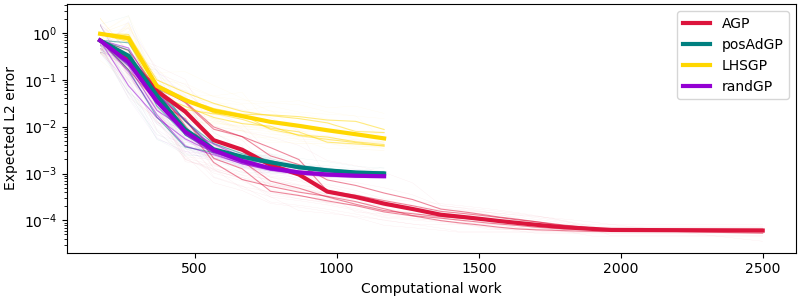
\includegraphics[width=0.8\textwidth]{results/pictures/d3/GP_res.png}
\end{center}
\caption{Convergence rates for the GPR expected error over computational budget for the four considered strategies on the 3d example and default configuration. The thinner lines represent a single run, the lines of median thickness represent the average over the 5 random seed for each measurement and the thickest lines represent the average over the whole 25 runs.}
\label{fig:3dGPconv}
\end{figure}

This setup results in the expected error per spent budget curves represented by Figure~\ref{fig:3dGPconv} for the different training strategies.
We see that, while \texttt{LHSGP} struggles to reduce the expected error and has a slower convergence rate, the fixed-tolerance strategies \texttt{posAdGP} and \texttt{randGP} are able to perform on par with \texttt{AGP} until they hit a plateau around an error level of $10^{-3}$, while \texttt{AGP} is able to reach the threshold $\texttt{tol}$ before the maximum number of iterations.
Moreover we observe that in this case random selection of the candidates in \texttt{randGP} is as effective as the position-adaptive strategy \texttt{posAdGP}, resulting in a similar convergence velocity.

\begin{table}[H]
    \begin{centering}
    \begin{tabular}{cccc}
    \toprule
         & Iterations & Training points & Computational work \\
         \midrule
         \texttt{AGP} 
         & 15.1 & 14.4 & 830 \\
         \texttt{posAdGP} 
         & 19.2 & 24.2 & 806 \\
         \texttt{randGP} 
         & 18.8 & 23.8 & 794  \\
         \bottomrule
    \end{tabular}
    \caption{Average over the 25 runs of number of iterations, points in the training set and computational work required to reduce the expected error below $2 \cdot 10^{-3}$ for the GPR-based adaptive strategies.}
    \label{tab:3dGP-plateau}
\end{centering}
\end{table}

As shown in Table~\ref{tab:3dGP-plateau}, while before the plateau \texttt{AGP} and the position-adaptive strategies achieve a similar performance in terms of expected error per budget, \texttt{AGP} uses a smaller number of iterations and training points as it adaptively reduces the default tolerance $\tau_d$ and optimizes work distribution.

\begin{table}[H]
    \begin{centering}
        
    
    \begin{tabular}{ccccccccccc}
    \toprule
        & Converged & $W$  & \multicolumn{4}{c}{Training points} & \multicolumn{4}{c}{Iterations} \\ 
        &   &  avg  & avg   & med   & min   & max   & avg   & med   & min   & max \\
        \midrule
        \texttt{AGP}, $\tau_d = 3 \cdot 10 ^{-2}$    
        &always & 1830 & 15.3  &  15   &  12   &  20   &  20.6 &  21   &   16  & 23   \\
        Others, $\tau_d = 3 \cdot 10 ^{-2}$    
        & never & 1167 &  35   &  35   &  35   &   35  &   30  &  30   &   30  & 30   \\
        \texttt{posAdGP}, $\tau_d = 10 ^{-3}$ 
        & always&14320 & 14.3  &  15   &  12   &   18  &  9.3  &  10   &   7   & 13   \\
        \texttt{randGP}, $\tau_d = 10 ^{-3}$ 
        & always&15080 & 15.1  &  14   &  14   &   17  &  8.1  &  9    &   9   & 12 \\
        \texttt{LHSGP}, $\tau_d = 10 ^{-3}$ 
        & never &35000 &  35   &  35   &  35   &   35  &   30  &   30  &   30  & 30   \\
    \bottomrule
    \end{tabular}
    \caption{Status of the training after the final iteration of different strategies and configurations for the GPR surrogate, 3d example. For the total computational work $W$ the average over the 25 runs is provided, while for the final number of points in the training set and the number of iterations necessary to terminate the training the average, the median, the minimum and the maximum are provided.
    }
    \label{tab:3dGP-recap}
\end{centering}
\end{table}

The plateau phase motivates us to test the behavior of the fixed-tolerance strategies with a lower tolerance $\tau_d = 10^{-3}$: in this case \texttt{posAdGP} and \texttt{randGP} are able to reach the target threshold $\texttt{tol}$ as shown in Figure~\ref{fig:3dGP-other}, but they require a larger computational budget and a similar number of training points as \texttt{AGP} with the lower default tolerance $\tau_d =  3\cdot 10^{-2}$, see Table~\ref{tab:3dGP-recap}.
We observe that even in this higher-accuracy case, \texttt{LHSGP} is unable to reach the convergence threshold \texttt{tol}.
Finally, on Table~\ref{tab:3dGP-recap} we can notice that on average a run \texttt{AGP} does not include the selected candidate in 10 iterations, resulting in an average number of 15.3 points in the design, of which 5 are the initial ones, over 20.6 average iterations.
As the computational costs of GPR scale with the number of training points, a reduced number of training points renders the evaluation of the surrogate more efficient.

\begin{figure}[H]
\begin{center}
    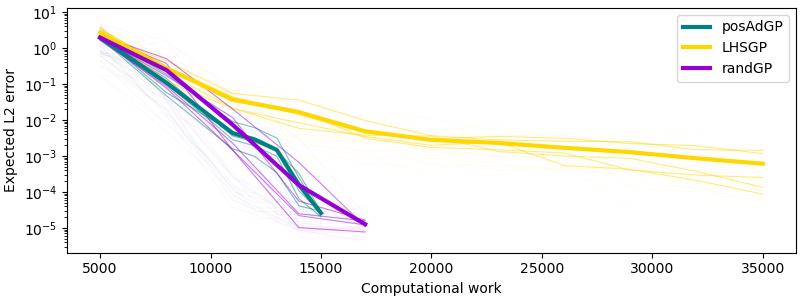
\includegraphics[width=0.8\textwidth]{results/pictures/d3/config_dtol0.001/GP_res.png}
\end{center}
\caption{Convergence rates for the GP expected error over computational budget for the fixed-tolerance strategies, default tolerance $\tau_d = 10^{-3}$. The thinner lines represent a single run, the lines of median thickness represent the average over the 5 random seed for each measurement and the thickest lines represent the average over the whole 25 runs.}
\label{fig:3dGP-other}
\end{figure}

For the LR surrogate, we consider a halting threshold $\texttt{tol} = \sigma \cdot \frac{\text{dim} \mc Y }{1.5} = 9.\bar 3 \cdot 10^{-2}$, proportional to the measurement's standard deviation as the error model is based on the standard deviation of the LR surrogate.
For LR, we sample every $N_{\text{sample}} = 4$ iterations and we set the number of walkers to $n_w = 32$.
The initial design consists of 5 points selected through LHS and with default tolerance $\tau_d = 3 \cdot 10^{-2}$, and we perform a maximum of $J_{\max} = 8 \cdot N_{\text{samples}} = 32$ iterations; when assigning the budget $\Delta W_j = \tau ^{-\frac{l}{r}}$ to the tolerance optimization problem at Step 3, we use the default value $\tau= \tau_d$ for the first $2\cdot N_{\text{samples}}= 8$ iterations and then every $N_{\text{sample}}$ iterations we halve it if the expected error has not reduced by a factor 2 compared to the $N_{\text{sample}}$-th latest iteration, i.e. if $\frac{E(D(\mc D_j))}{E(D(\mc D_{j-N_{\text{sample}}}))} > \frac{1}{2}$.
The different choices regarding configuration parameters as compared to GPR are due to the higher prediction variance and lower sensitivity of the LR surrogate model to computational work. 

\begin{figure}[H]
\begin{center}
    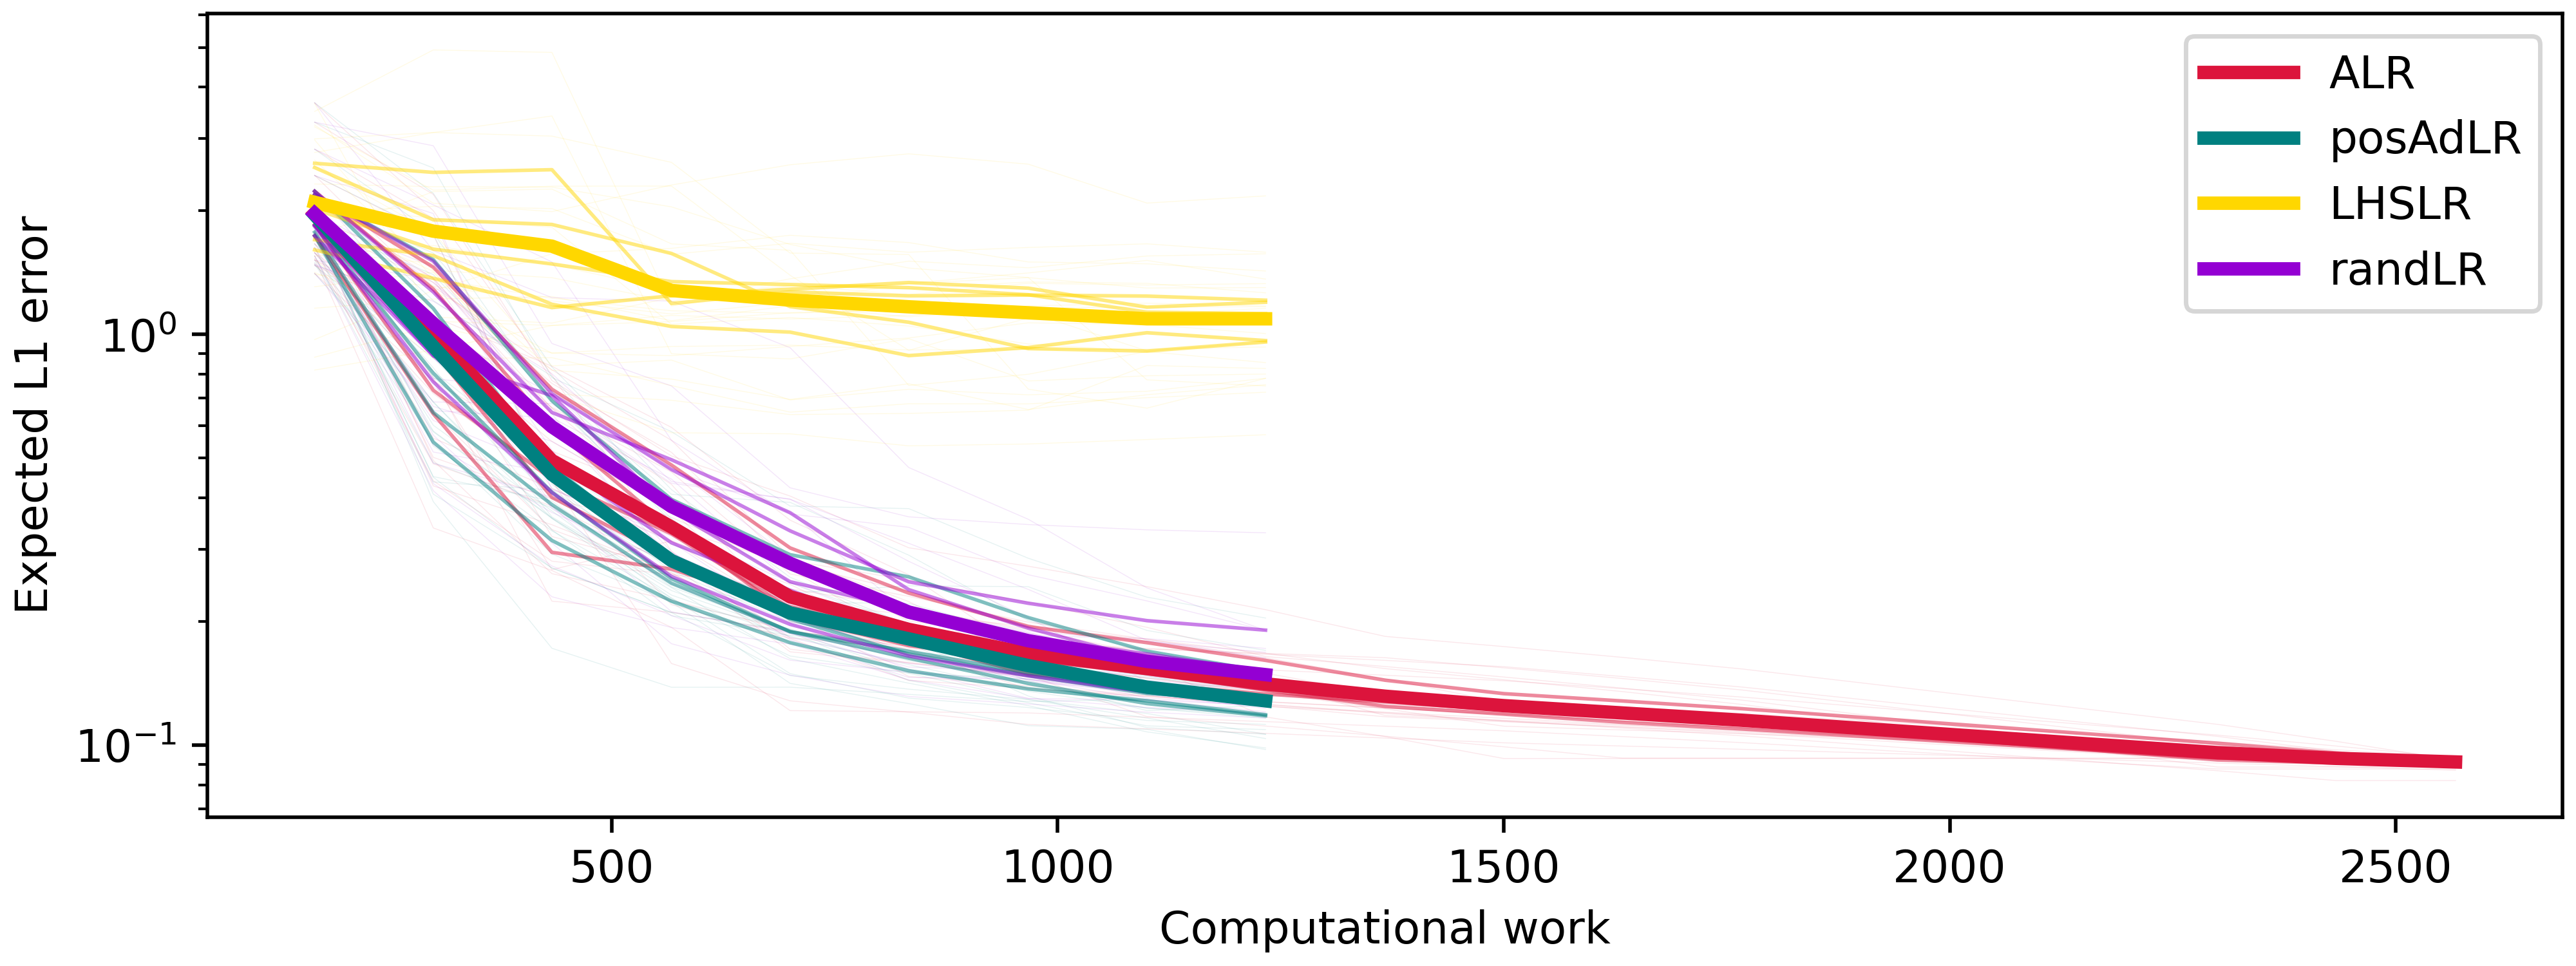
\includegraphics[width=0.8\textwidth]{results/pictures/d3/LR_res.png}
\end{center}
\caption{Convergence rates for the LR expected error over computational budget for the four considered strategies. The thinner lines represent a single run, the lines of median thickness represent the average over the 5 random seed for each measurement and the thickest lines represent the average over the whole 25 runs.}
\label{fig:3dLRconv}
\end{figure}

Figure~\ref{fig:3dLRconv} depicts the expected error per budget curves for the different training strategies. 
We observe that, as opposed to the GPR surrogate, the fixed-tolerance strategies \texttt{posAdLR} and \texttt{randLR} perform on par with \texttt{ALR} until they meet the maximum number of iterations, while \texttt{ALR} is able to reach the target threshold $\texttt{tol}$ before the maximum number of iterations thanks to the adaptive budget allocation.
It is worth noting that \texttt{LHSLR} performs significantly worse than the other strategies, barely reducing the expected error at all, while \texttt{posAdLR} performs slightly better than \texttt{randLR}. 
In this case, the fully adaptive strategy \texttt{ALR} includes the new candidate in the design more frequently than \texttt{AGP}, resulting in an average for the 25 runs of 27.1 training points over 26.4 iterations, corresponding on average to around 4 iterations without the inclusion of the candidate.
This fact, as well as the effectiveness of fixed-tolerance strategies, suggests that for LR the inclusion of high-accuracy points is a less relevant factor than in GPR on this example. \medskip

\begin{table}[H]

    \begin{centering}
        
    \hspace*{-1.5cm}
    \begin{tabular}{ccccccccccccc}
    \toprule
        & \multicolumn{4}{c}{MAP error}  & \multicolumn{4}{c}{Posterior mean error} & \multicolumn{4}{c}{Posterior st. dev. error} \\ 
        & \multicolumn{4}{c}{$ \|p_\text{MAP} - \hat p _\text{MAP}\|_2 $}  & \multicolumn{4}{c}{$ \|p_\text{mean} - \hat p _\text{mean}\|_2 $} & \multicolumn{4}{c}{$\| \text{diag}(\Sigma_P) - \text{diag}( \hat \Sigma _P) \|_2$} \\ 
        & avg   & med   & min   & max   & avg   & med   & min   & max   & avg   & med   & min   & max \\
        \midrule
        \texttt{AGP}
        & 0.0046 & 0.0039 & 0.0011 & 0.0086
        & 0.0037 & 0.0036 & 0.0011 & 0.0084
        & 0.0038 & 0.0015 & 0.0001 & 0.0131 \\
        \texttt{posAdGP}
        & 0.0145 & 0.0152 & 0.0048 & 0.0214 
        & 0.0136 & 0.0141 & 0.0049 & 0.0217
        & 0.0071 & 0.0067 & 0.0034 & 0.0110 \\
        \texttt{randGP}
        & 0.0103 & 0.0097 & 0.0048 & 0.0192 
        & 0.0107 & 0.0106 & 0.0041 & 0.0201
        & 0.0064 & 0.0058 & 0.0011 & 0.0136 \\
        \texttt{LHSGP}
        & 0.0332 & 0.0325 & 0.0124 & 0.0753 
        & 0.0312 & 0.0278 & 0.0119 & 0.0658
        & 0.0149 & 0.0131 & 0.0088 & 0.0331 \\
        \texttt{ALR}
        & 0.0186 & 0.0180 & 0.0041 & 0.0446
        & 0.0113 & 0.0102 & 0.0043 & 0.0272
        & 0.0094 & 0.0087 & 0.0024 & 0.0196 \\
        \texttt{posAdLR}
        & 0.0199 & 0.0178 & 0.0041 & 0.0524
        & 0.0139 & 0.0115 & 0.0037 & 0.0369
        & 0.0103 & 0.0095 & 0.0049 & 0.0208 \\
        \texttt{randLR}
        & 0.0225 & 0.0211 & 0.0077 & 0.0507
        & 0.0156 & 0.0141 & 0.0053 & 0.0283
        & 0.0117 & 0.0113 & 0.0052 & 0.0232 \\
        \texttt{LHSLR}
        & 0.1315 & 0.1134 & 0.0536 & 0.2801 
        & 0.1053 & 0.0992 & 0.0319 & 0.1988
        & 0.0717 & 0.0707 & 0.0251 & 0.1378 \\
        
    \bottomrule
    \end{tabular}

    \caption{Average, median, minimum and maximum of the absolute error on the MAP estimate, posterior mean and posterior standard deviation on each component over the 25 runs with default configuration.
    The analytical ground truth posterior and corresponding samples are utilized to compute the true MAP $p_\text{MAP}$, mean $p_\text{mean}$ and component-wise standard deviation $\text{diag}(\Sigma_P)$, while for each strategy the surrogate-based posteriors and samples are used to compute $\hat p_\text{MAP}$, $\hat p_\text{mean}$ and $\text{diag}(\hat \Sigma_P)$.
    }
    \label{tab:3d-comparison}
    \end{centering}
    
    
\end{table}

We compare the performance of the GPR and LR surrogates utilizing the available ground truth.
Table~\ref{tab:3d-comparison} shows the average error on the MAP estimate, posterior mean and posterior standard deviation of the different strategies and different surrogates.
First, we observe that the GPR-based strategies perform significantly better than the LR-based ones, with \texttt{AGP} being the best performing strategy across all metrics with a precision of one order of magnitude better than others on the MAP and mean errors. 
The tolerance-adaptive strategy \texttt{ALR} performs at a level similar to that of \texttt{posAdGP} and \texttt{randGP}, but with a higher computational cost.
As already noticed with the expected error per budget curves, the difference among \texttt{ALR} and the LR-based fixed-tolerance strategies is less pronounced than for GPR.
In fact, in the fixed-tolerance strategies LR is able to reach a performance at the same order of magnitude as GPR by having a locally-accurate representation of the forward model with a similar computational cost.
We can notice that the LHS-based strategies \texttt{LHSGP} and \texttt{LHSLR} are worst performing ones and display a remarkable performance difference between the two surrogate kinds. 
In this example, LR is unable to obtain a good approximation of the posterior through a globally-accurate surrogate, while GPR is able to reach a good approximation of the posterior even with a non-adaptive globally-accurate surrogate.
\begin{figure}[t]
\begin{center}
    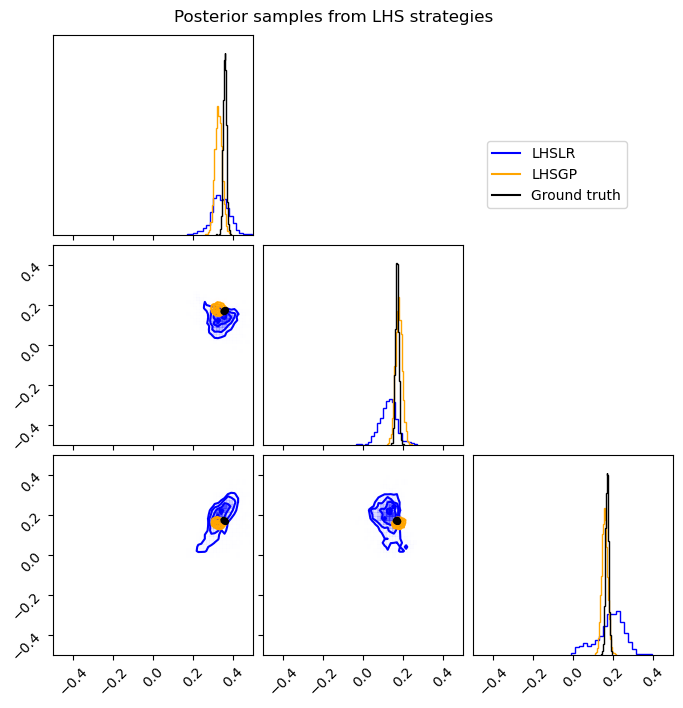
\includegraphics[width=0.8\textwidth]{results/pictures/d3/LHS_samples4_0.png}
\end{center}
\caption{Final sample chains from \texttt{LHSGP} and \texttt{LHSLR}, default tol $\tau_d = 3\cdot 10^{-2}$, compared with the ground truth for the run with the 5-th measurement set and pseudorandom seed 0.}
    \label{fig:3d-LHS}
\end{figure}
Figure~\ref{fig:3d-LHS} plots the samples gathered from the posteriors from \texttt{LHSGP} and \texttt{LHSLR} as well as the ground truth for one of the runs.




\subsection{6d analytical example - Diffusion equation}\label{sec:6dexp}

The second numerical experiment involves the homogeneous diffusion equation on $\R^3$ with unit diffusivity constant and no source
\[
\partial_t u - \Delta u =0,
\]
and initial conditions given by two Dirac's delta of opposite sign centered in some $x_p$ and $x_n$:
\[
f (0,x; x_p, x_n) = \delta(x-x_p) - \delta(x-x_n).
\]
We consider the difference of fundamental solutions of the diffusion equation centered in $x_p$ and $x_n$, scaled for numerical stability of the surrogates, as a solution of the above problem
\begin{equation}\label{eq:diffusion-solution}
f(t,x; x_p, x_n) = \frac{50}{(4 \pi t)^{\frac{3}{2}}} \left( \exp \left( - \frac{\norm{x-x_p}_2^2}{4t}\right)- \exp \left( - \frac{\norm{x-x_n}_2^2}{4t}\right) \right).
\end{equation}
We treat $x_p, x_n$ as unknown parameters and want to identify them by measuring $u(t,x;x_p, x_n)$ for $t,x \in \mc S$, where $\mc S$ is a set of times in $\R^+$ coupled with sensors in $\R^3$ given by
\[
\mc S  = \left\{ (t,x) \in \R^+ \times \R^3 \ \Big| \ t = 0.3, 0.5 \ \text{ and } \ x = \begin{pmatrix}
            \cos( i \frac{2\pi}{3}) \sin( j \frac{\pi}{4}) \\
            \sin( i \frac{2\pi}{3}) \sin( j \frac{\pi}{4}) \\ 
            \cos( j \frac{\pi}{4})
        \end{pmatrix} 
         \text{ for } i \in \{0,1,2\}, \ j \in \{0,1,2,3,4\}
        \right\}.         
\]
This results in 15 sensors at 2 different times, resulting in a 30-dimensional measurement space $\mc Y = \R^{30}$. \newline
As a parameter space, $\Omega = [-1,1]^6$ is considered and a Normal prior $\mc N (0, \frac{1}{4}I_6)$ is assumed.
Measurements are generated by exact forward model evaluations $y(p)$ for 4 different values of $p$ randomly extracted from the prior distribution, to which pseudorandom noise $N \sim \mc N (0, \sigma^2 I_{30})$, with $\sigma = 2 \cdot 10^{-2}$ is added.
For each of the 4 measurements, we perform 3 runs of each training strategy with different random seeds. \medskip

The configuration parameters for the GPR surrogate are similar to those of the previous example: we choose an halting threshold of $\texttt{tol} = \sigma^2 \cdot \frac{\text{dim} \mc Y }{20} = 6\cdot 10^{-4}$; sampling is performed every $N_{\text{sample}} = 4$ iterations, with an ensemble comprising of $n_w = 64$ walkers.
The initial design consists of 13 points selected through LHS with default tolerance $\tau_d = 3 \cdot 10^{-2}$; we perform a maximum of $J_{\max} = 10 \cdot N_{\text{samples}} = 40$ iterations and at Step 3 of the algorithm we assign $\Delta W_j = \tau ^{-\frac{l}{r}}$ computational budget, using the default value $\tau= \tau_d$ for the first $2\cdot N_{\text{samples}} = 8$ iterations and then again halving it every $N_{\text{sample}}$ iterations if the expected error has not reduced by a factor 4 compared to the $N_{\text{sample}}$-th latest iteration, i.e. if $\frac{E(D(\mc D_j))}{E(D(\mc D_{j-N_{\text{sample}}}))} > \frac{1}{4}$.

\begin{figure}[H]
\begin{center}
    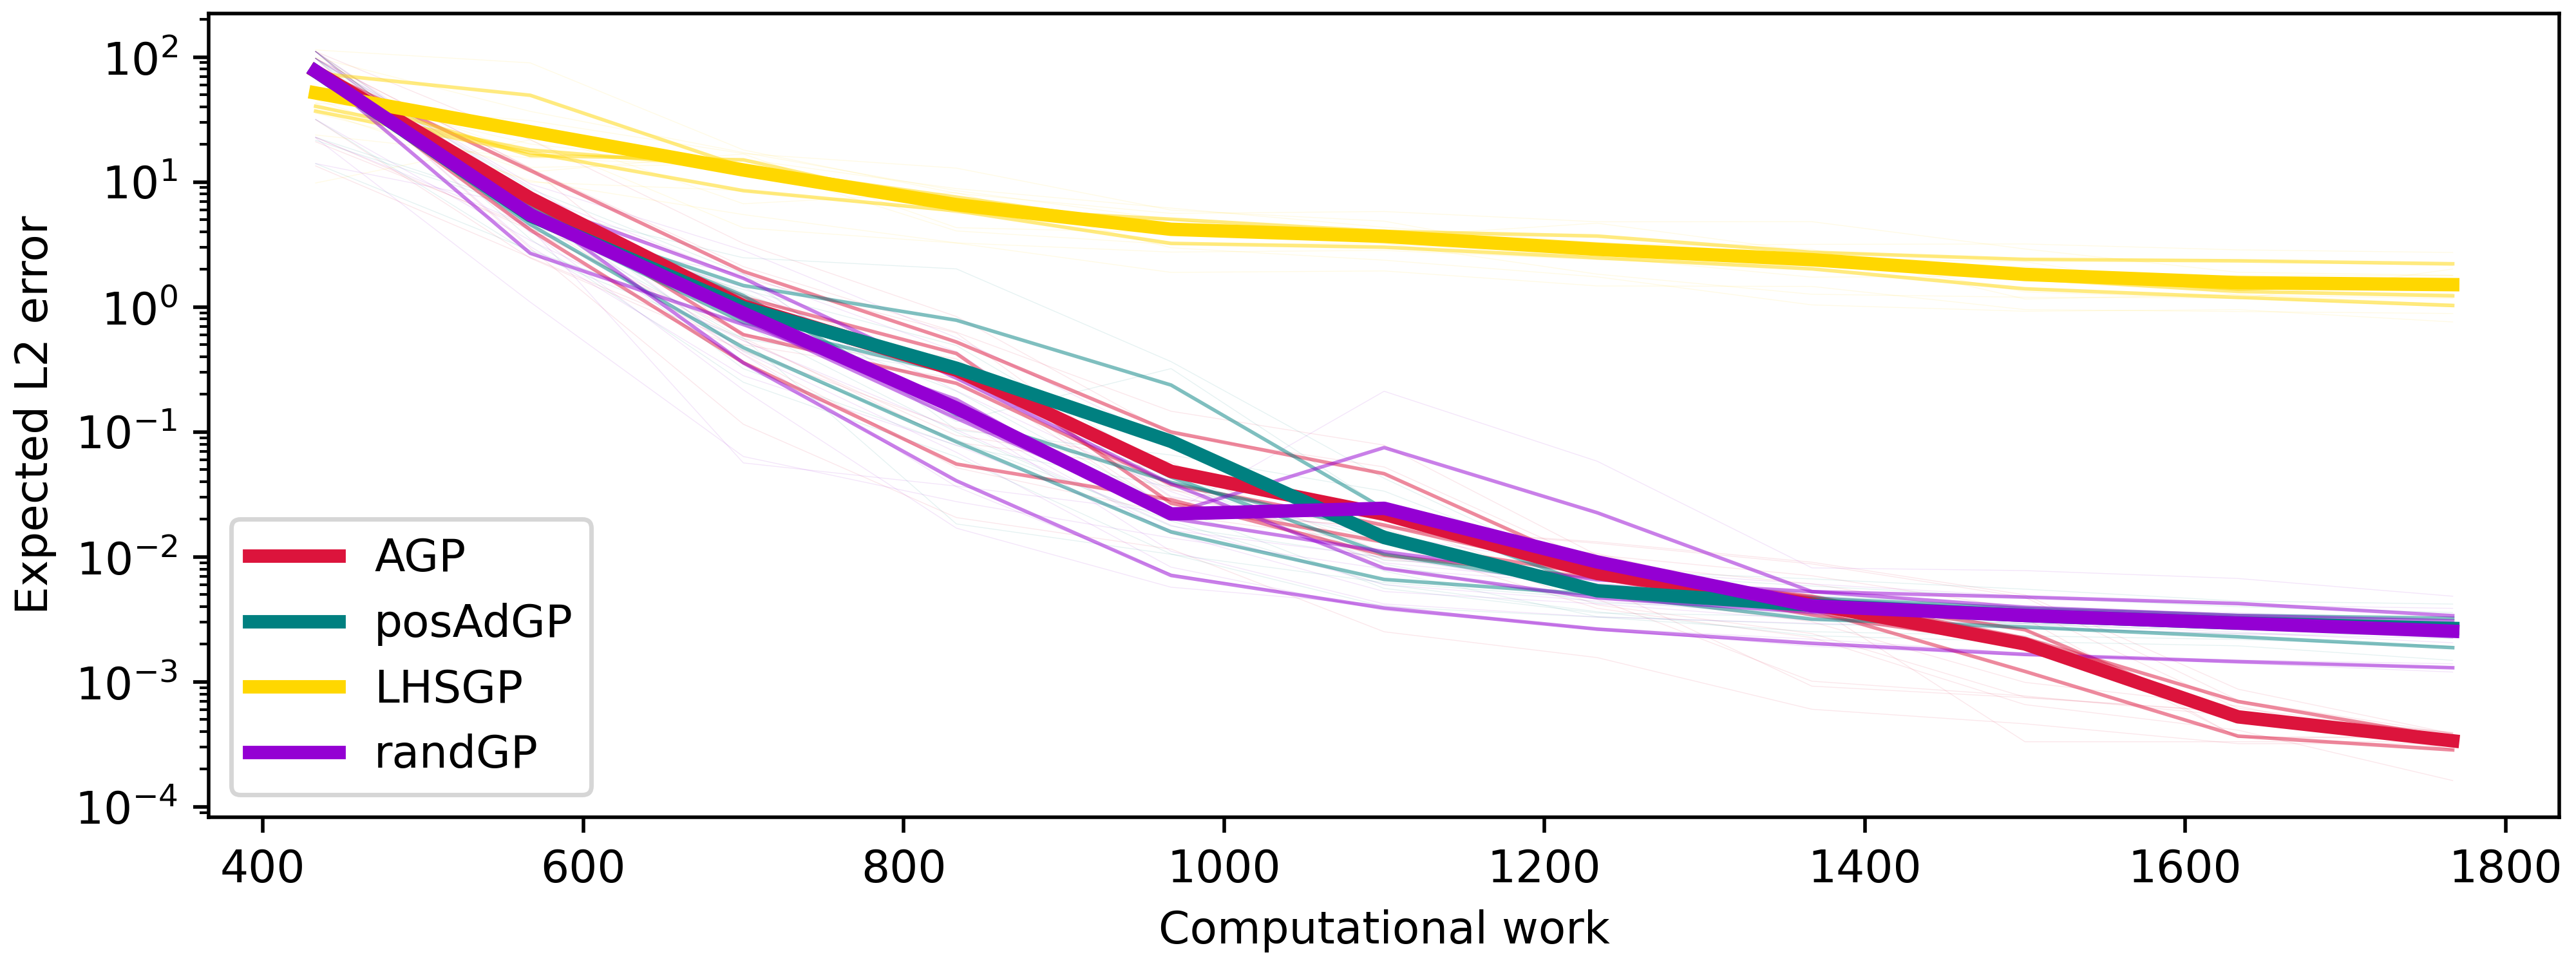
\includegraphics[width=0.8\textwidth]{results/pictures/d6/GP_res.png}
\end{center}
\caption{Convergence rates for the GP expected error over computational budget for the four considered strategies on the 6d example. The thinner lines represent a single run, the lines of median thickness represent the average over the 4 random seed for each measurement and the thickest lines represent the average over the whole 12 runs.}
    \label{fig:6dGPconv}
\end{figure}

The convergence curves resulting from the different training strategies with the above configuration are shown in Figure~\ref{fig:6dGPconv}.
In this example, we observe that, despite an overall higher error level, the relative performance of the different strategies is similar to the previous experiment; the position-adaptive strategies \texttt{posAdGP} and \texttt{randGP} stall at an error level of $10^{-3}$, while \texttt{AGP} is able to reach the target threshold $\texttt{tol}$ before the maximum number of iterations and \texttt{LHSGP} is unable to reduce the expected error significantly.
In contrast to the previous example, \texttt{AGP} is closer to the fixed-tolerance strategies \texttt{posAdGP} and \texttt{randGP} in terms of expected error per budget, but also spends considerably less budget than the previous experiment: both of these effects can be due to the higher likelihood standard deviation $\sigma$, here set to $2\cdot 10^{-2}$ in contrast to $10^{-2}$ in the previous example, which possibly makes the need for higher-accuracy evaluations less pressing.
This can also be seen in the lower number of iterations where no new candidate is selected, as shown in Table~\ref{tab:6dGP-recap}.
Another considerable difference is that \texttt{LHSGP} performs significantly worse than the other strategies, likely due to the higher dimensionality of the parameter space which makes evenly spaced sampling less effective.

\begin{table}[H]
    \begin{centering}
    \begin{tabular}{ccccc}
    \toprule
        & $E$   & $W$ & Training points    & Iterations \\ 
        \midrule
        \texttt{AGP}  
        & 0.0003 & 1734 & 31.9  &  23.1   \\
        \texttt{posAdGP}
        & 0.0021 & 1767 & 53    & 40   \\
        \texttt{randGP}
        & 0.0019 & 1767 & 53    & 40 \\
        \texttt{LHSGP}
        & 1.1770 & 1767 &  53   & 40   \\
    \bottomrule
    \end{tabular}
    \caption{Status of the training after the final iteration of different strategies for the GPR surrogate, 6d example. The average values over the 12 runs for the final error level $E$, total computational work $W$, the final number of points in the training set and the number of iterations necessary to terminate the training are provided.
    }
    \label{tab:6dGP-recap}
\end{centering}
\end{table}

For the LR we tried default configuration parameters similar to the previous one: after setting the halting threshold to $\texttt{tol} = \sigma \cdot \frac{\text{dim} \mc Y }{1.5} = 0.6$, we sampled every $N_{\text{sample}} = 5 $ iterations and set the number of walkers to $n_w = 64$.
The initial design consists of 13 points selected through LHS with default tolerance $\tau_d = 3 \cdot 10^{-2}$; we perform a maximum of $J_{\max} = 8 \cdot N_{\text{samples}} = 40$ iterations and at Step 3 of the algorithm we assign $\Delta W_j = \tau ^{-\frac{l}{r}}$ computational budget, using the default value $\tau= \tau_d$ for the first $2\cdot N_{\text{samples}}= 10$ iterations and then again halving it every $N_{\text{sample}}$ iterations if the expected error has not reduced by a factor 2 compared to the $N_{\text{sample}}$-th latest iteration, i.e. if $\frac{E(D(\mc D_j))}{E(D(\mc D_{j-N_{\text{sample}}}))} > \frac{1}{2}$.

This setup resulted in a poor performance for all strategies, as shown in Figure~\ref{fig:6dLRconv}, with \texttt{LHSLR} performing the worst but also the adaptive strategies \texttt{ALR}, \texttt{posAdLR} and \texttt{randLR} being unable to reduce the expected error significantly; moreover in the last iterations \texttt{ALR} spends considerably more budget than the fixed-tolerance strategies, resulting in a total computational work of 6766 for all of the runs as it tries to adaptively reduce the default tolerance $\tau_d$ but the expected error does not reduce correspondingly.
To try to improve the performance, we tried to lower the default tolerance $\tau_d$ to $10^{-3}$ and consider more iterations with $N_{\text{sample}} =  6$ and $J_{\max} = 9 \cdot N_{\text{sample}} $ in order to improve the results of all strategies, but this did not significantly improve the overall performance of any the considered strategies resulting in a lower error level but with convergence curves similar to the ones depicted in Figure~\ref{fig:6dLRconv}; despite the higher computational budget all strategies and runs were unable to reach the threshold \texttt{tol} and achieve convergence, with even the better runs not obtaining an error level below 1.

\begin{figure}[H]
\begin{center}
    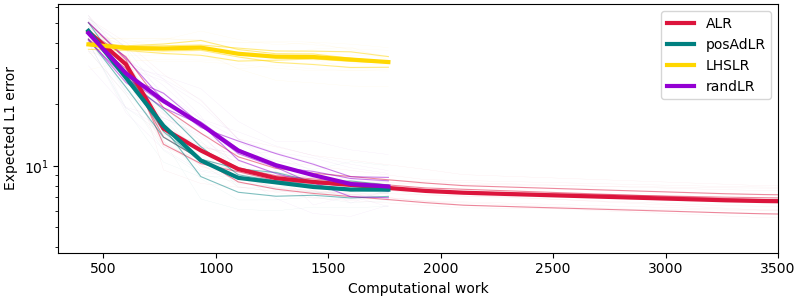
\includegraphics[width=0.8\textwidth]{results/pictures/d6/LR_res.png}
\end{center}
\caption{Convergence rates for the LR expected error over computational budget for the four considered strategies on the 6d example. The thinner lines represent a single run, the lines of median thickness represent the average over the 4 random seed for each measurement and the thickest lines represent the average over the whole 12 runs. The computational budget axis was truncated at 3300 as the budget spent by \texttt{ALR} far exceeds the ones from other strategies. }
    \label{fig:6dLRconv}
\end{figure}


The failure of LR on this problem can be attributed to the nature of the forward model; in fact, due to the rapid decay of the solution~\eqref{eq:diffusion-solution}, the steepness of every component varies greatly over the parameter space, and moreover the flatter and steeper regions are distinct for each component.
For a component $j$ of $y$, let $(t,x)$ being the corresponding time and sensor position.
Then, the Lipschitz constant for $y^{(j)}(x_p,x_n) = f(t,x;x_p,x_n)$ is given by 
\begin{align*}
    L^{(j)} = \max_{(x_p,x_n)\in\Theta}& \left\| \partial_{x_p,  x_n} y^{(j)}(x_p,x_n) \right\|_\infty  =
    \max_{x_p\in[-1,1]^3} \left\| \partial_{x_p} f(t,x;x_p,0) \right\|_\infty  =\\
    &\qquad \qquad= \max_{x_p\in [-1,1]^3} \left| \frac{50}{(4 \pi t)^{\frac{3}{2}}}\exp \left( - \frac{\norm{x-x_p}_2^2}{4t}\right) \frac{x^{(1)}-x_p^{(1)}}{4t} \right| 
    = \frac{100}{(8\pi)^{\frac{3}{2}}} e^{-\frac{1}{2}} t^{-2},
\end{align*}
where for symmetry reasons we can consider the derivative with respect to the first component of $x_p$ only, as the maximum is the same for all components of $\partial_{x_p, x_n} f(t,x;x_p,x_n)$, being obtained for component $h$ of $\partial_{x_p} f(t,x;x_p,x_n)$ in $x_p = x \pm \sqrt{2t} \cdot e_h$, with $e_h$ being the $h-$th vector of the canonical base of $\R^3$, and similarly for $x_n$.
Note that for any $(t,x) \in \mc S$ and $h \in \{1,2,3\}$, one between $(x + \sqrt{2t} e_h, \tilde x)$ and $(x - \sqrt{2t} e_h, \tilde x)$ is inside $\Theta$ for any $\tilde x \in [-1,1]^3$.

For $t=0.3$ and $t=0.5$ this results in a ground-truth global Lipschitz constant of approximately $ 5.3$ and $1.9$ for the respective components of the surrogate model.
However, in all components the minimum value of the local Lipschitz constant can go well below 0.1, and large portions of the parameter space can be covered with a significantly smaller Lipschitz constant.
This kind of behavior is extremely difficult to capture with a LR surrogate, which considers a global Lipschitz constant for every component of the forward model, as the surrogate requires a great number of points in order to be able to reduce the uncertainty of its prediction in the flatter region of each component.\medskip

The comparison of the performance of the GPR and LR surrogates is shown in Table~\ref{tab:6d-comparison}, where we can see that the performance of GPR is considerably better than that of LR; the best performance from an LR-based strategy is the one from \texttt{ALR}: but even for the fully-adaptive strategy strategy the corresponding estimates are unreliable and substantially wrong, and result being around as accurate as the ones provided by \texttt{LHSGP} for a smaller computational cost.
Regarding GPR-based strategies, two observations can be made.
First, the actual error values confirm the behavior suggested by the expected error curves, with the gap between \texttt{AGP} and the fixed-tolerance strategies being smaller, and the performance of \texttt{LHSGP} being far worse than in the 3d case.
Second, we can notice that while the median values achieved by \texttt{randGP} are on par with the other adaptive strategies, there is a considerably high maximum value for the error on the MAP and mean estimates.
As the standard deviation error does not display such phenomenon, this indicates that in some run \texttt{randGP} was misled and converged to the wrong posterior.

\begin{table}

    \begin{centering}
        
    
    \hspace*{-1.5cm}
    \begin{tabular}{ccccccccccccc}
    \toprule
        & \multicolumn{4}{c}{MAP error}  & \multicolumn{4}{c}{Posterior mean error} & \multicolumn{4}{c}{Posterior st. dev. error} \\ 
        & \multicolumn{4}{c}{$ \|p_\text{MAP} - \hat p _\text{MAP}\|_2 $}  & \multicolumn{4}{c}{$ \|p_\text{mean} - \hat p _\text{mean}\|_2 $} & \multicolumn{4}{c}{$\| \text{diag}(\Sigma_P) - \text{diag}( \hat \Sigma _P) \|_2$} \\ 
        & avg   & med   & min   & max   & avg   & med   & min   & max   & avg   & med   & min   & max \\
        \midrule
        \texttt{AGP}
        & 0.0086 & 0.0075 & 0.0029 & 0.0219
        & 0.0046 & 0.0036 & 0.0016 & 0.0105
        & 0.0935 & 0.0812 & 0.0657 & 0.1400 \\
        \texttt{posAdGP}
        & 0.0211 & 0.0164 & 0.0027 & 0.0637
        & 0.0270 & 0.0138 & 0.0013 & 0.1783
        & 0.0860 & 0.0845 & 0.0336 & 0.1383 \\
        \texttt{randGP}
        & 0.0511 & 0.0117 & 0.0051 & 0.3140
        & 0.0392 & 0.0062 & 0.0034 & 0.3378
        & 0.0998 & 0.0845 & 0.0336 & 0.1860 \\
        \texttt{LHSGP}
        & 0.2960 & 0.3019 & 0.1498 & 0.4543 
        & 0.2535 & 0.2439 & 0.0854 & 0.4684
        & 0.1229 & 0.1248 & 0.0226 & 0.2303 \\
        \texttt{ALR}
        & 0.3017 & 0.3139 & 0.1830 & 0.4252
        & 0.3021 & 0.3030 & 0.1383 & 0.4348
        & 0.0653 & 0.0657 & 0.0259 & 0.1099 \\
        \texttt{posAdLR}
        & 0.4045 & 0.3933 & 0.1955 & 0.6292
        & 0.3902 & 0.3541 & 0.1867 & 0.5732
        & 0.0655 & 0.0496 & 0.0191 & 0.1144 \\
        \texttt{randLR}
        & 0.5490 & 0.5420 & 0.3975 & 0.7604
        & 0.5563 & 0.5361 & 0.3867 & 0.7746
        & 0.0492 & 0.0423 & 0.0167 & 0.1089\\
        \texttt{LHSLR}
        & 0.6616 & 0.6180 & 0.3113 & 1.0597
        & 0.6257 & 0.6539 & 0.3246 & 0.9277
        & 0.2767 & 0.2836 & 0.0717 & 0.4703\\
        
    \bottomrule
    \end{tabular}
    \caption{Average, median, minimum and maximum of the absolute error on the MAP estimate, posterior mean and component-wise posterior standard deviation on each component over the 12 runs with default configuration.
    As for Table~\ref{tab:3d-comparison} the analytically available ground truth is used to compute the true quantities $p_\text{MAP}$, $p_\text{mean}$ and $\Sigma_P$, which are then compared with the surrogate-based estimates $\hat p_\text{MAP}$, $\hat p_\text{mean}$ and $\hat \Sigma_P$.
    }
    \label{tab:6d-comparison}
\end{centering}
\end{table}

\subsection{2d Finite Element example - Elastomechanics}\label{sec:FEexp}
For the third numerical experiment we consider a 2d elastomechanics problem, based on the equations of linear elasticity as introduced at the end of Section~\ref{sec:AdaFE}.
We consider a rectangular beam of length $L=4 m$ and quadratic cross-section of equal height and width $h=w=0.2 m$, constrained on the left and right sides, with a uniform downward load applied on the top side.
This conditions correspond to a Dirichlet boundary condition on the left and right sides, an inhomogeneous Neumann boundary condition on the top side and a homogeneous Neumann boundary condition on the rest of the beam.
Formally, our spatial domain is
\[
    \mc X = [0,L] \times [0,h] ^2 \in \R^3
\]
and we consider the homogeneous version of the Lamè-Navier equations~\eqref{eq:Navier-Lame} over $\mc X$
\[
    -2\mu \Delta u - \lambda \nabla (\nabla \cdot u) = 0,
\]
for Lamè parameters $\lambda, \mu$; the boundary conditions are given by
\[
    \begin{cases}
        u(x,y,z) = 0 & \text{ if } x = 0, L \\
        \partial_n u(x,y,z) = F & \text{ if } y = h \\
        \partial_n u(x,y,z) = 0 & \text{ otherwise}
    \end{cases}
\]
where $F = -5\cdot 10^6$ is a dimensionless quantity corresponding to a uniform load on the top.
We aim at identifying the Young's modulus $E$ and the Poisson's ratio $\nu$ of the material as given by Equation~\eqref{eq:material-parameters}.
We consider sensors placed in the center of the beam on the different sides, one at the top, one at the bottom, one on the left and one on the right
\[
    \mc S = \left\{ (2,0,0.1), (2,0.2,0.1), (2,0.1,0), (2,0.1,0.2) \right\} 
\]
and in each sensor we measure one component of the displacement field $u$ at the corresponding position: the vertical component for the top and bottom sensors and the horizontal component for the left and right sensors.
This results in a 4-dimensional measurement space $\mc Y = \R^4$ and a measurement operator \[
 \begin{gathered}
    H : H^1(\mc X;\R^3) \to \mc Y \\
    H(u) = S \begin{pmatrix}
     u^{(2)}(2,0,0.1)\\
     u^{(2)}(2,0.2,0.1)\\
     u^{(3)}(2,0.1,0)\\
     u^{(3)}(2,0.1,0.2) 
    \end{pmatrix} + a \in \R^4,
 \end{gathered}
\]
where the scaling diagonal matrix $S = \text{diag}(s_1, s_2, s_3, s_4)$ and the offset vector $a = (a_1,a_2,a_3,a_4)$ are added in order to center the model response into $[0,1]^4$.
We assume an original parameter space 
\[
    \hat \Omega = [90 \ GPa, 300 \ GPa] \times [0.1, 0.45] \subset \R^2 
\]
which for numerical stability we scale to $\Omega = [0,1]^2$ through an affine transformation.
As the forward model's image over the parameter space is in the order of $10^{-2}$ for the first two components and $10^{-6}$ for the last two, we set the scaling factors to $s_1 = s_2 = - \frac{100}{6}$ and $s_3 = - s_4 = 4 \cdot 10^5$ and the offset to $a_1 = a_2 = \frac{6}{100}$ and $a_3 = - a_4 = - 5 \cdot 10^{-7}$. \newline
We assume a Normal prior $\mc N(\frac{1}{2}, \frac{1}{6}I_2)$ over $\Omega$ and we consider a ground truth value for the parameters of $\hat p = (200 \ GPa, 0.25) \in \hat \Omega$, which are the material parameters of A36 steel.
The measurements are then generated by adding pseudorandom noise $N \sim \mc N (0, \sigma^2 I_4)$ with $\sigma = 10^{-2}$ to the forward model evaluation $y_\tau (p)$ for $p\in \Omega$ corresponding to the ground truth parameters $\hat p$ and with a tolerance of $\tau = 10^{-4}$.
Unlike the analytical examples, where we performed multiple runs in order to average over the randomly added noise, in this case we only perform one run for each strategy and surrogate, as the forward model is an actual FE model with non-negligible computational costs. \medskip

For the GPR surrogate we consider a default configuration similar to the one of the preceding examples, with the difference that we consider a default tolerance $\tau_{d,a}= 10^{-2}$ for the fully-adaptive \texttt{AGP} strategy and a default tolerance $\tau_{d,f} = 10^{-3}$ for the fixed-tolerance strategies.
We set the halting threshold to $\texttt{tol} = \sigma^2 \cdot \frac{\text{dim} \mc Y }{20} = 2\cdot 10^{-5}$, while sampling every $N_{\text{sample}} = 2$ iterations with an ensemble composed of $n_w = 16$ walkers.
For each strategy, the initial design comprises of $3$ points selected through LHS and evaluated with the default tolerance corresponding to the strategy; we perform a maximum of $J_{\max} = 10 \cdot N_{\text{samples}} = 20 $ iterations.
For the tolerance problem in \texttt{AGP}, we assign the budget $\Delta W_j = \tau ^{-\frac{l}{r}}$ using the default value $\tau= \tau_{d,a}$ for the first $2\cdot N_{\text{samples}} = 4$ iterations and then every $N_{\text{sample}}$ iterations we have $\tau$ if the expected error has not reduced by a factor 4 compared to the $N_{\text{sample}}$-th latest iteration, i.e. if $\frac{E(D(\mc D_j))}{E(D(\mc D_{j-N_{\text{sample}}}))} > \frac{1}{4}$.\medskip

\begin{figure}[H]
    \begin{center}
        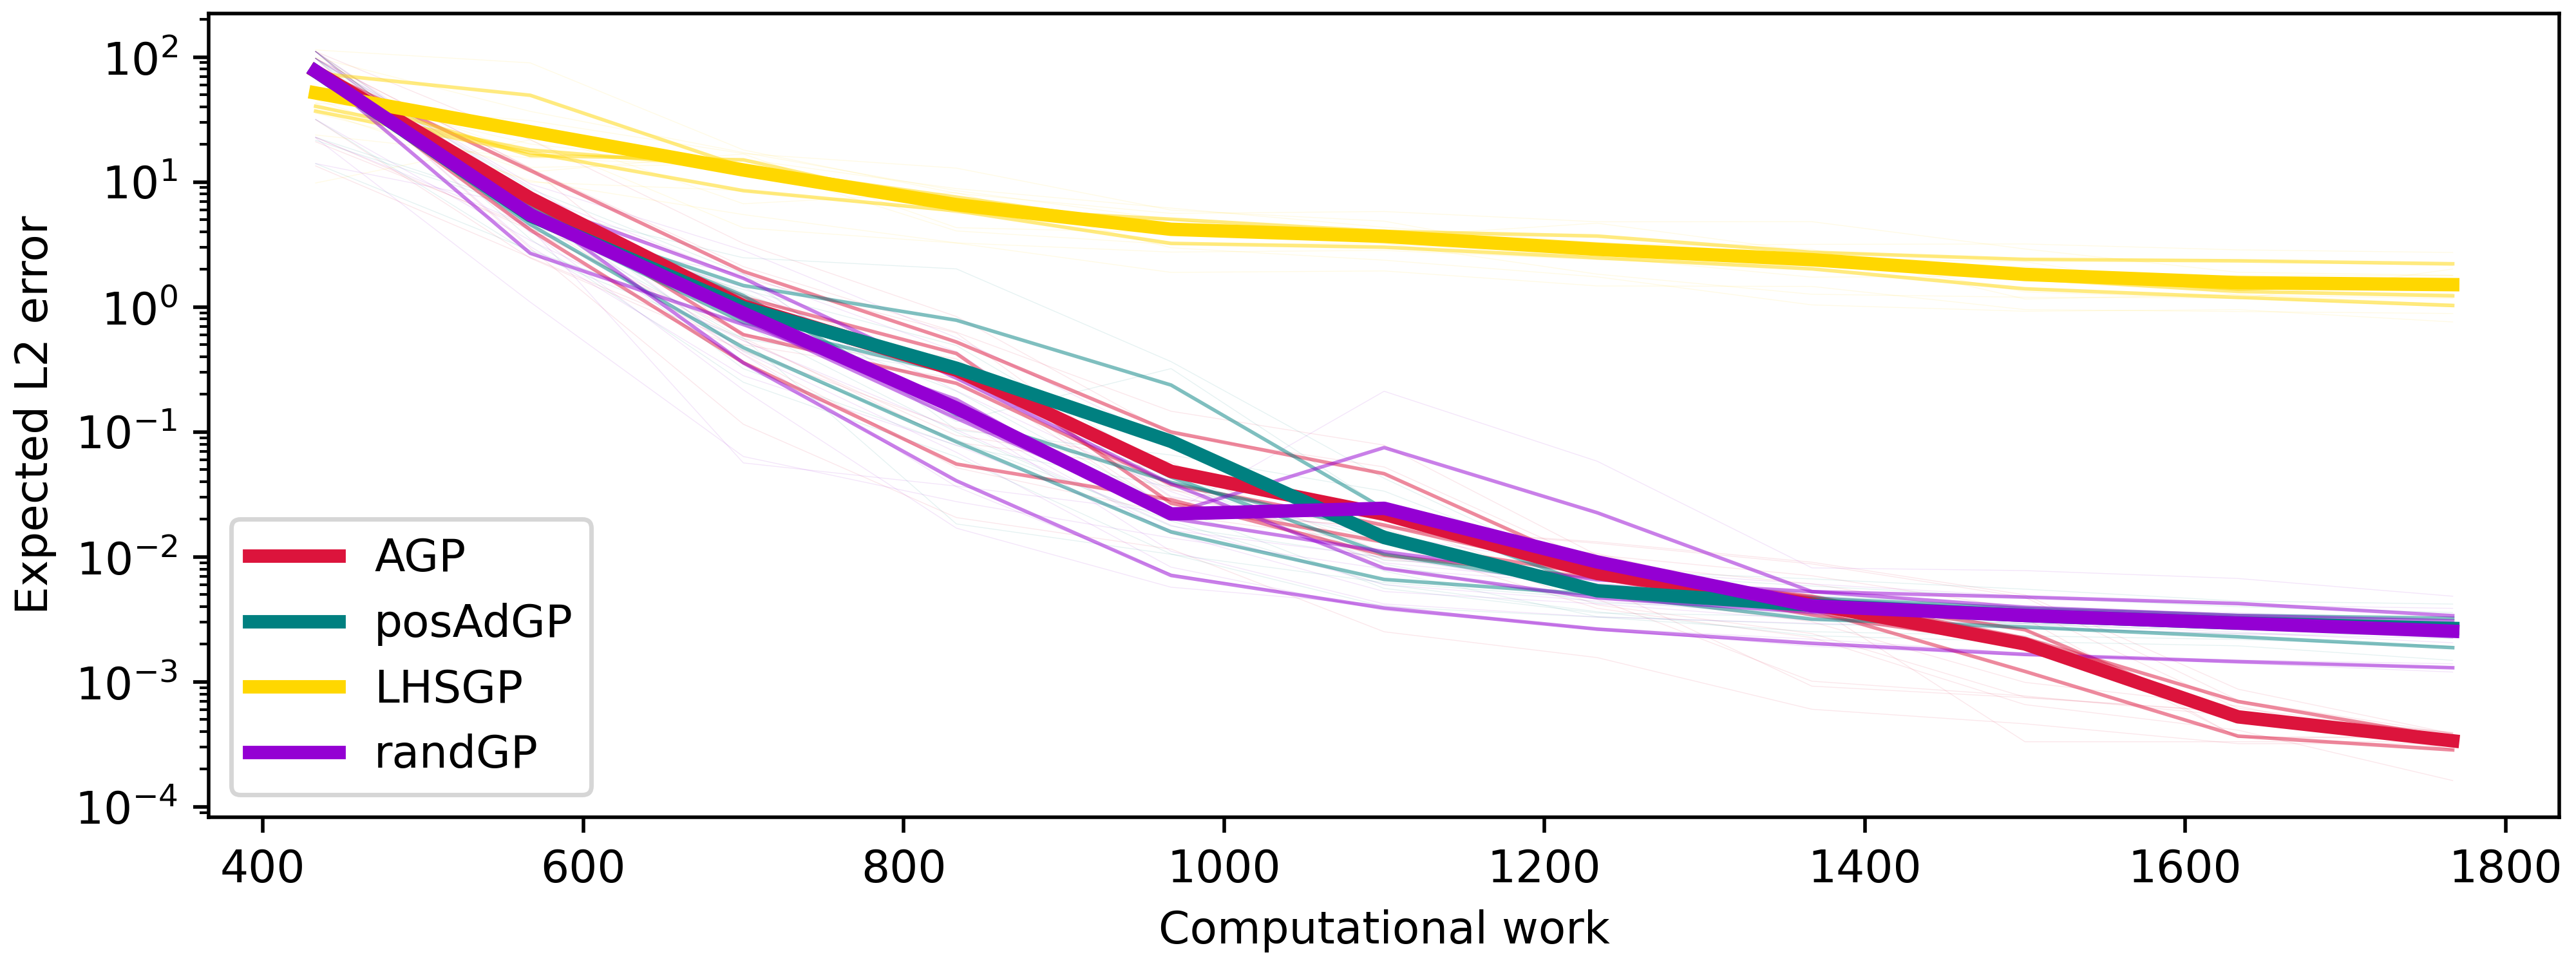
\includegraphics[width=0.8\textwidth]{results/pictures/d6/GP_res.png}
    \end{center}
    \caption{Convergence rates for the GP expected error over computational budget for the four considered strategies on the 2d FE example. A single line is plotted as a single measurement with a single random seed is used for each strategy.}
        \label{fig:FE-GP-convergence}
\end{figure}

Picture~\ref{fig:FE-GP-convergence} depicts the convergence curves for the GPR expected error over computational budget for the different strategies, while Table~\ref{tab:FE-GP-recap} summarizes the status of the training after the final iteration of the different strategies.
We observe that all strategies reach the halting threshold before the maximum number of iterations, included \texttt{LHSGP}; this success from the LHS-based strategy is likely due to the low dimensionality of the parameter space, which allows for a good coverage of the parameter space with relatively few points.
Moreover, we can see that \texttt{AGP} is able to reach the halting threshold with a significantly lower computational budget and similar number of points than the fixed-tolerance strategies.
Finally, we note that \texttt{randGP} performs worse than the other adaptive strategies, almost on the level of \texttt{LHSGP}.
\begin{table}[H]
    \begin{centering}
    \begin{tabular}{ccccc}
    \toprule
        & converged   & $W$ & Training points    & Iterations \\ 
        \midrule
        \texttt{AGP}  
        & yes & 252823 &  17   &  16  \\
        \texttt{posAdGP}
        & yes & 442719 &  15   &  11  \\
        \texttt{randGP}
        & yes & 600833 &  19   &  16  \\
        \texttt{LHSGP}
        & yes & 727324 &  21   &  18  \\
    \bottomrule
    \end{tabular}
    \caption{Status of the training after the final iteration of different strategies for the GPR surrogate, FE example. For the single run performed the convergence status, total computational work $W$, the final number of points in the training set and the number of iterations necessary to terminate the training are provided.
    }
    \label{tab:FE-GP-recap}
\end{centering}
\end{table} 
Picture~\todo{fig:FE-GP-samples} shows the samples gathered from the different strategies as well as the ground truth value utilized to generate the measurements.\medskip

For the LR surrogate we do similarly as done for the GPR surrogate, utilizing diffrent tolerances for the fully-adaptive strategy \texttt{ALR} and the fixed-tolerance strategies \texttt{posAdLR}, \texttt{randLR} and \texttt{LHSLR}; we use a default tolerance $\tau_{d,a}= 10^{-2}$ for \texttt{ALR} and a default tolerance $\tau_{d,f} = 10^{-3}$ for the others.
The halting threshold is set to $\texttt{tol} = \sigma \cdot \frac{\text{dim} \mc Y }{1.5} = 2.\bar 6 \cdot 10^{-2}$, we sample every $N_{\text{sample}} = 3$ iterations and set the number of walkers to $n_w = 16$.
The initial design consists of $5$ points selected through LHS with the default tolerance corresponding to the strategy; we perform a maximum of $J_{\max} = 7 \cdot N_{\text{samples}} = 21 $ iterations and for the tolerance problem at Step 3 of the algorithm for \texttt{ALR} we assign $\Delta W_j = \tau ^{-\frac{l}{r}}$ using the default value $\tau= \tau_{d,a}$ for the first $2\cdot N_{\text{samples}} = 6$ iterations and then every $N_{\text{sample}}$ iterations we have $\tau$ if the expected error has not reduced by a factor 2 compared to the $N_{\text{sample}}$-th latest iteration, i.e. if $\frac{E(D(\mc D_j))}{E(D(\mc D_{j-N_{\text{sample}}}))} > \frac{1}{2}$.\medskip

\begin{figure}[H]
    \begin{center}
        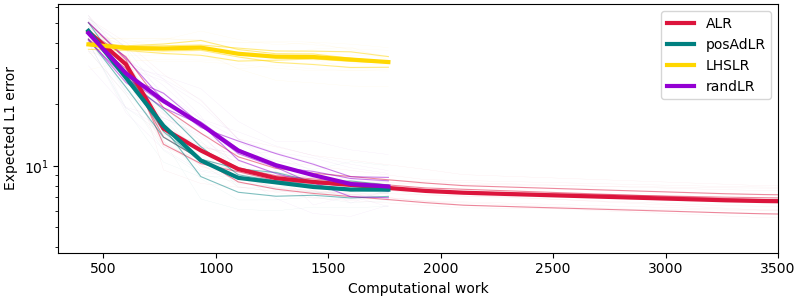
\includegraphics[width=0.8\textwidth]{results/pictures/d6/LR_res.png}
    \end{center}
    \caption{Convergence rates for the LR expected error over computational budget for the four considered strategies on the 2d FE example. A single line is plotted as a single measurement with a single random seed is used for each strategy.}
        \label{fig:FE-LR-convergence}
\end{figure}

The expected error over computational budget curves for the LR surrogate are shown in Picture~\ref{fig:FE-LR-convergence}; like for the GPR-based strategies we observe that all strategies reach the halting threshold before the maximum number of iterations, included \texttt{LHSLR}.
Table~\ref{tab:FE-LR-recap} summarizes the status of the training after the final iteration of the different strategies.
\begin{table}[H]
    \begin{centering}
    \begin{tabular}{cccccc}
    \toprule
        & converged   & E & $W$ & Training points    & Iterations \\ 
        \midrule
        \texttt{AGP}  
        & no & 0.0857 & 846425 &  25   &  21  \\
        \texttt{posAdGP}
        & no & 0.1092 & 822192 &  26   &  21 \\
        \texttt{randGP}
        & no & 0.1777 & 822192 &  26   &  21 \\
        \texttt{LHSGP}
        & no & 0.4887 & 822192 &  26   &  21 \\
    \bottomrule
    \end{tabular}
    \caption{Status of the training after the final iteration of different strategies for the GPR surrogate, FE example.
    }
    \label{tab:FE-LR-recap}
\end{centering}
\end{table} 

Finally, Picture~\todo{fig:FE-LR-samples} shows the samples gathered from the different strategies and the groung truth value $p$ employed to generate the measurements.




\subsection[Effects of covariance estimation]{Effects of the discretization noise covariance's estimation}\label{sec:cov-est}

To test the impact of the estimation of the discretization noise covariance $\Sigma_D^2$ on the performance of the surrogate, we utilize the data from the 3-d and 6-d analytical examples, where the discretization noise covariance is known.
First we test the absolute error on the matrix 2-norm of the shrinkage covariance estimate $\hat \Sigma_D^2$ defined in Equation~\eqref{eq:shrinkage-estimator}; second, we test the effect of considering $\tau \hat \Sigma_D^2$ instead of diagonal noise $\tau I_{\text{dim}\mc Y}$ in GPR~\eqref{eq:GP-predictive} by training two GPR surrogates with the two covariances and then comparing the predictive variance of the surrogates over the parameter space and he resulting MAP and mean estimates as well as the corresponding posteriors standard deviation.





%%%%%%%%%%%%%%%%%%%%%%%%%%%%
%%%%%%%%%%%%%%%%%%%%%%%%%%%%


\newpage
\pagestyle{fancyapp}
\appendix
\section{Appendix A: Gaussian process regression}\label{app:GPR}
Here we provide the proof of Theorem~\ref{thm:GP-posterior}.
\GPpost*
\begin{proof}
    Let $p,p' \in \Theta$ be two prediction points, and let $Y_{\hat{P} } = (Y_{p_1}, \ldots, Y_{p_n}, Y_p, Y_{p'})$. 
    We will derive the joint posterior distribution for $Y_{\hat{P}}$ by Bayes theorem and then obtain the mean predictiom for $Y_p$ and the covariance between $Y_p$ and $Y_{p'}$ by exploiting some linear algebra results. \\
    By \textit{(GPR-model)}, the 

\end{proof}

\section{Appendix B: derivatives for the GPR acquisition function}\label{app:derivatives} 
\todo[inline]{update notation}
We consider a design $\left( (p_i,\tau_i)\right)_{i=1,\dots,s}$ and a GP kernel $k$. Using the explicit formula for the predictive variance given in~\cite[equation 2.24]{RasmussenWilliams2006}, the derivative of $\Gamma(p)$ with respect to $\tau_i$ is given by \[
    \frac{\partial \Gamma(p)}{\partial \tau_i} = 2\tau_i K_* (K + \mathfrak{T} ^2  )^{-1} (I_m \otimes \text{diag}(e_i))(K + \mathfrak{T} ^2  )^{-1} K_*^T,
\] 
where $\underline{e_1}, \dots,\underline{e_s}$ is the canonical basis of $\R^s$, and the kernel matrices are\[
K = \begin{bmatrix} k(p_1,p_1) & \dots & k(p_1,p_s) \\
    \vdots               & \ddots & \vdots \\
    k(p_s,p_1) & \dots & k(p_s,p_s)
\end{bmatrix} \ \text{ and } \
K_* =  \begin{bmatrix}
    k(p_1,p) \\
    \vdots \\
    k(p_s,p)
\end{bmatrix}.
\]
The derivative is obtained by considering the work model and inverting it:
\[
\frac{\partial \tau}{\partial W} = -\frac{r}{l} W^{-\frac{r}{l}-1}.
\]

\section{Appendix B: Expected error reduction}\label{app:EER}

Here we provide the proof of Proposition~\ref{prp:EER}.
\EER*
\begin{proof}
We recall that Equation~\eqref{eq:alpha-LR-general} defines the expected error reduction as
\[
    \alpha_{\mc D, \text{LR}}(p, p') = 
    \bb E _{ (Y_p, \nu) \sim \mc U( \mc PI_p \times  [-\tau_p, \tau_p] ^{ \text{dim} \mc Y } )} 
    \left[ 
        e_{D(\mc D), \text{LR}}(p')- e_{D(p,\tau_p, Y_p + \nu ), \text{LR}}(p')
    \right],
\]
and in the hypothesis of the proposition we have that $\mc PI_p$ is a multivariate interval with lower and upper bounds given by Equations~\eqref{eq:LR-bounds}.\newline
As $\mc PI_p$ is a multivariate interval, we can use Equation~\eqref{eq:loc-err-LR} and have for every training set $D$, $p\in \Theta$
\[
    e_{D, \text{LR}}(p) = \frac{1}{2\sqrt{3}} \sum_{j=1}^{\text{dim}\mc Y} \left( UB_{D}^{(j)}(p) - LB_{D}^{(j)}(p) \right),
\]
where we added the subscript $D'$ to the bounds as in this proposition there are different training sets involved, and we will continue to do so in the rest of the proof.\newline
Then, we have that 
\begin{flalign*}
    e_{D(\mc D), \text{LR}}(p')&- e_{D(p,\tau_p, Y_p + \nu ), \text{LR}}(p') = \\
    &= \frac{1}{2\sqrt{3}} \sum_{j=1}^{\text{dim}\mc Y} \left(  \left( UB_{D(\mc D)}^{(j)}(p') - UB_{D(p,\tau_p, Y_p + \nu )}^{(j)}(p') \right) - \left( LB_{D(\mc D)}^{(j)}(p') - LB_{D(p,\tau_p, Y_p + \nu )}^{(j)}(p') \right) \right),
\end{flalign*}
which we insert in the expression of $\alpha_{\mc D, \text{LR}}(p, p')$ to obtain, after using the linearity of the expectation operator, the following equality:
\begin{flalign}
    \alpha_{\mc D, \text{LR}}(p, p') = \frac{1}{2\sqrt{3}} \sum_{j=1}^{\text{dim}\mc Y}\Big( &\bb E _{ (Y_p, \nu) \sim \mc U\left( \mc PI_p \times  [-\tau_p, \tau_p] ^{ \text{dim} \mc Y } \right)} \left[  \left( UB_{D(\mc D)}^{(j)}(p') - UB_{D(p,\tau_p, Y_p + \nu )}^{(j)}(p') \right)\right] - \label{eq:EER-proof-1} &&\\
    & \qquad - \bb E _{ (Y_p, \nu) \sim \mc U\left( \mc PI_p \times  [-\tau_p, \tau_p] ^{ \text{dim} \mc Y } \right)} \left[  \left( LB_{D(\mc D)}^{(j)}(p') - LB_{D(p,\tau_p, Y_p + \nu )}^{(j)}(p') \right) \right]\Big). &&\notag
\end{flalign}
BY observing that as $\mc PI_p$ is an interval all the components of $(Y_p,\nu)$ are independent, and that both $UB_D^{(j)}$ depends on the $j$-th component of the training data only, we can write 
\begin{flalign*}
    &\bb E _{ (Y_p, \nu) \sim \mc U\left( \mc PI_p \times  [-\tau_p, \tau_p] ^{ \text{dim} \mc Y } \right)} \left[  \left( UB_{D(\mc D)}^{(j)}(p') - UB_{D(p,\tau_p, Y_p + \nu )}^{(j)}(p') \right)\right] = && \\
    & \qquad\qquad =\bb E _{ \left(Y_p^{(j)}, \nu^{(j)}\right) \sim \mc U\left( \left[LB^{(j)}_{D(\mc D)}(p), UB^{(j)}_{D(\mc D)}(p)\right] \times  [-\tau_p, \tau_p] \right)} \left[  \left( UB_{D(\mc D)}^{(j)}(p') - UB_{D(p,\tau_p, Y_p + \nu )}^{(j)}(p') \right)\right] = &&\\
    & \qquad\qquad = \frac{1}{2\tau_p \left(  UB^{(j)}_{D(\mc D)}(p)- LB^{(j)}_{D(\mc D)}(p) \right) } \int_{UB^{(j)}_{D(\mc D)}(p)}^{LB^{(j)}_{D(\mc D)}(p)} \int_{-\tau_p}^{\tau_p} UB_{D(\mc D)}^{(j)}(p') - UB_{D(p,\tau_p, y + n )}^{(j)}(p') \,dn \, dy &&\\
    & \qquad\qquad \eqcolon \frac{ EUI^{(j)}(p,p')}{2\tau_p \left(  UB^{(j)}_{D(\mc D)}(p)- LB^{(j)}_{D(\mc D)}(p) \right) }  &&,
\end{flalign*}
and similarly for the term with the lower bounds, resulting in the integral term $ELI^{(j)}(p,p')$.\newline
By inserting the above in Equation~\eqref{eq:EER-proof-1} and factoring out $\frac{1}{2\tau_p}$, we obtain that Equation~\eqref{eq:loc-err-LR} holds (note that in the statement $UB$ and $LB$ do not have any subscript, but they are what we are denoting with $UB_{D(\mc D)}$ and $LB_{D(\mc D)}$ respectively).\newline
We now need to compute the integrals $EUI^{(j)}(p,p')$ and $ELI^{(j)}(p,p')$: due to symmetry reasons (the lower bound is the negative of the upper bound resulting from data with a change of sign $\tilde y^{(j)} = - y^{(j)} $), it suffices to compute $EUI$ only.\newline
By Equations~\eqref{eq:LR-bounds} and by the fact that $D(p,\tau_p, Y_p + \nu ) = D (\mc D) \cup \{ (p, \tau_p, Y_p + \nu ) \}$, we have that \[
    UB_{D(p,\tau_p, Y_p + \nu )}^{(j)}(p') = \min \left( UB_{D(\mc D)}^{(j)}(p'), Y_p +\nu + \tau_p + L^{(j)} \|p'-p \|_\Theta \right),
\]
allowing us to write 
\[
    EUI^{(j)}(p,p') = \int_{LB^{(j)}_{D(\mc D)}(p)}^{UB^{(j)}_{D(\mc D)}(p)} \int_{-\tau_p}^{\tau_p} \max \left( 0, UB_{D(\mc D)}^{(j)}(p') - y -n - \tau_p - L^{(j)} \|p'-p \|_\Theta \right) \,dn \, dy.
\]


We collect the constant terms in the constant $c_1^j = UB^{(j)}_{D(\mc D)}(p') - \tau_p - L^{(j)} \|p'-p \|_\Theta$. 
The treatment of the integral depends on the interplay between $c_1^j$, $UB^{(j)}_{D(\mc D)}(p)$, $LB^{(j)}_{D(\mc D)}(p)$ and $\tau_p$, as the integrand is $0$ whenever $y> c_1 -n$.
As an integration order will be more convenient in some cases and less convenient in others, we treat the cases separately.
Note that as $UB^{(j)}_{D(\mc D)}(p) \geq LB^{(j)}_{D(\mc D)}(p)$, some more inequalities will be left implicit.
Pictures~\ref{fig:cases} depicts the considered cases, with each colored line representing an instance of the line $y = c_1^j - n$ in the case corresponding to the associated number.

\begin{figure}[H]
    \begin{centering}
        \includesvg[width = 0.7\textwidth]{results/pictures/integration domain}
    \caption{Example of the integration domain with the line $y = c_1^j - n$ above which the integrand is 0 for the cases 1-6 described below.} 
    \label{fig:cases} 
    \end{centering}
\end{figure}  
The cases considered are the following:\medskip

\textbf{Case 1:} $UB^{(j)}(p) \leq c_1^j - \tau_p $. \smallskip \newline
As $UB^{(j)}(p) +\tau_p \leq c_1^j$, we have \[
    \max \left( 0, c_1^j - y - n \right) = c_1^j - y - n \ \text{ for all } \ (y,n) \in \left[LB^{(j)}_{D(\mc D)}(p), UB^{(j)}_{D(\mc D)}(p)\right] \times [-\tau_p, \tau_p],
\] 
thus 
\begin{flalign*}
    EUI^{(j)}(p,p') &= \int_{LB^{(j)}_{D(\mc D)}(p)}^{UB^{(j)}_{D(\mc D)}(p)} \int_{-\tau_p}^{\tau_p} c_1^j - y - n \,dn \, dy = && \\
    &= c_1^j \cdot 2 \tau_p \cdot \left( UB^{(j)}_{D(\mc D)}(p) - LB^{(j)}_{D(\mc D)}(p) \right) - 2 \tau_p \cdot \frac{1}{2} \left( UB^{(j)}_{D(\mc D)}(p)^2 - LB^{(j)}_{D(\mc D)}(p)^2 \right) = &&\\
    &= \tau_p \left( UB^{(j)}_{D(\mc D)}(p) - LB^{(j)}_{D(\mc D)}(p) \right) \left( 2 c_1^j - UB^{(j)}_{D(\mc D)}(p) - LB^{(j)}_{D(\mc D)}(p) \right)   &&
\end{flalign*}
holds as stated. \medskip
% case 5 on paper

\textbf{Case 2:} $c_1^j + \tau_p < UB^{(j)}(p) $ and $ LB^{(j)}(p) \leq c_1^j - \tau_p$. \smallskip \newline
As we have that 
\begin{equation}\label{eq:EER-proof-2}
    \max \left( 0, c_1^j - y - n \right) = 0 \ \text{ for all } \ (y,n) \ \text{ such that } \ y + n \geq c_1^j,
\end{equation}
holds, in this case we write the integral as
\begin{flalign*}
    EUI^{(j)}(p,p') &= \int_{-\tau_p}^{\tau_p} \int_{LB^{(j)}_{D(\mc D)}(p)}^{c_1^j - n}  c_1^j - y - n \,dy \, dn = && \\
    &= \int_{-\tau_p}^{\tau_p} \left( c_1^j - n \right) \cdot \left( c_1^j - n - LB^{(j)}_{D(\mc D)}(p) \right) - \frac{1}{2} \left( \left( c_1^j - n \right)^2 - LB^{(j)}_{D(\mc D)}(p)^2 \right) \, dn = && \\
    &= \int_{-\tau_p}^{\tau_p} \frac{1}{2} \left( c_1^j - n  - LB^{(j)}_{D(\mc D)}(p)\right)^2  \, dn = && \\
    &= \frac{1}{6 }\left( \left( c_1^j + \tau_p  - LB^{(j)}_{D(\mc D)}(p)\right)^3 - \left( c_1^j - \tau_p  - LB^{(j)}_{D(\mc D)}(p)\right)^3 \right), &&
\end{flalign*}
which is the desired result. \medskip
%case 1 on paper 

\textbf{Case 3:} $c_1^j + \tau_p < UB^{(j)}(p) $ and $ c_1^j - \tau_p < LB^{(j)}(p) \leq c_1^j + \tau_p$. \smallskip \newline
In this case we use Equation~\eqref{eq:EER-proof-2} and write the following equalities
\begin{flalign*}
    EUI^{(j)}(p,p') &= \int_{-\tau_p}^{c_1^j - LB^{(j)}_{D(\mc D)}(p)} \int_{LB^{(j)}_{D(\mc D)}(p)}^{c_1^j - n}  c_1^j - y - n \,dy \, dn = && \\
    &= \int_{-\tau_p}^{LB^{(j)}_{D(\mc D)}(p)} \left( c_1^j - n \right) \cdot \left( c_1^j - n - LB^{(j)}_{D(\mc D)}(p) \right) - \frac{1}{2} \left( \left( c_1^j - n \right)^2 - LB^{(j)}_{D(\mc D)}(p)^2 \right) \, dn = && \\
    &= \int_{-\tau_p}^{LB^{(j)}_{D(\mc D)}(p)} \frac{1}{2} \left( c_1^j - n  - LB^{(j)}_{D(\mc D)}(p)\right)^2  \, dn = && \\
    &= \frac{1}{6 } \left( c_1^j + \tau_p  - LB^{(j)}_{D(\mc D)}(p)\right)^3 
\end{flalign*}
which deal the stated result.\medskip
%case 2 on paper 

\textbf{Case 4:} $ c_1^j - \tau_p < UB^{(j)}(p) \leq c_1^j + \tau_p$ and $ c_1^j - \tau_p < LB^{(j)}(p) \leq c_1^j + \tau_p$. \smallskip \newline
In this case Equation~\eqref{eq:EER-proof-2} renders it convenient to write the integral as
\begin{flalign*}
    EUI^{(j)}(p,p') &= \int_{LB^(j)_{D(\mc D)}(p)}^{UB^{(j)}_{D(\mc D)}(p)} \int_{-\tau_p}^{c_1^j - y}  c_1^j - y - n \,dn \, dy = && \\
    &= \int_{LB^{(j)}_{D(\mc D)}(p)}^{UB^{(j)}_{D(\mc D)}(p)} \left( c_1^j - y \right) \cdot \left( c_1^j - y + \tau_p \right) - \frac{1}{2} \left( \left( c_1^j - y \right)^2 - \tau_p^2 \right) \, dy = && \\
    &= \int_{LB^{(j)}_{D(\mc D)}(p)}^{UB^{(j)}_{D(\mc D)}(p)} \frac{1}{2} \left( c_1^j - y  + \tau_p\right)^2  \, dy = && \\
    &= \frac{1}{6 } \left(\left( c_1^j - LB^{(j)}_{D(\mc D)}(p) + \tau_p  \right)^3 - \left( c_1^j - UB^{(j)}_{D(\mc D)}(p) - \tau_p  \right)^3 \right), &&
\end{flalign*}
which implies the equality in the statement.\medskip
%case 3 on paper

\textbf{Case 5:} $ c_1^j - \tau_p < UB^{(j)}(p) \leq c_1^j + \tau_p $ and $ LB^{(j)}(p) \leq c_1^j - \tau_p$. \smallskip \newline
In this case, in order to solve the integral we have to split the domain in two:
\begin{flalign*}
    EUI^{(j)}(p,p') &= \int_{LB^{(j)}_{D(\mc D)}(p)}^{c_1^j - \tau_p} \int_{-\tau_p}^{\tau_p}  c_1^j - y - n \,dn \, dy + \int_{c_1^j - \tau_p}^{UB^{(j)}_{D(\mc D)}(p)} \int_{-\tau_p}^{c_1^j - y}  c_1^j - y - n \,dn \, dy = && \\
    &= 2\tau_p \int_{LB^{(j)}_{D(\mc D)}(p)}^{c_1^j - \tau_p}  c_1^j - y \,dy + \int_{c_1^j - \tau_p}^{UB^{(j)}_{D(\mc D)}(p)} \frac{1}{2} \left( c_1^j - y  + \tau_p\right)^2  \, dy = && \\
    &= 2\tau_p \left( c_1^j \left(c_1^j - \tau_p - LB^{(j)}_{D(\mc D)}(p) \right) + \frac{1}{2} \left(LB^{(j)}_{D(\mc D)}(p)^2 - (c_1^j - \tau_p)^2 \right) \right) - && \\
    & \qquad \qquad \qquad \qquad \qquad \qquad \qquad \qquad  - \frac{1}{6 } \left(\left( c_1^j - UB^{(j)}_{D(\mc D)}(p) + \tau_p  \right)^3 - 8 \tau_p^3 \right) &&
\end{flalign*}
holds, dealing the desired equality. \medskip
%case 4 on paper

\textbf{Case 6:} $c_1^j + \tau_p  < LB^{(j)}(p)$. \smallskip \newline
As $LB^{(j)}(p) -\tau_p > c_1^j$, we have that 
\[
    \max \left( 0, c_1^j - y - n \right) = 0 \ \text{ for all } \ (y,n) \in \left[LB^{(j)}_{D(\mc D)}(p), UB^{(j)}_{D(\mc D)}(p)\right] \times [-\tau_p, \tau_p],
\]
so the integral is zero as stated\medskip

The above cases deal the expression for $EUI$ provided in the statement, concluding the proof.
\end{proof}


\newpage
\pagestyle{fancybib}
\section*{Bibliography}
\bibliographystyle{plain}
\renewcommand\refname{}

\bibliography{references}
\addcontentsline{toc}{section}{Bibliography}

\end{document}

